\documentclass[12pt, a4paper, twoside, openright]{book}

\usepackage{vuwthesis} % sets up some local things, mostly the front page

\usepackage{palatino} % sets palatino as the default font

\usepackage{url} % for typesetting urls

\usepackage{graphicx}
\usepackage{amsmath}
\usepackage{amssymb}
\usepackage{hyperref}
\usepackage{csquotes}
\usepackage{epigraph}
\usepackage{wrapfig}
\usepackage{xcolor}
\usepackage{algorithm}
\usepackage[noend]{algpseudocode}
\usepackage[utf8x]{inputenc}
\DeclareUnicodeCharacter{2212}{-}
\providecommand{\tightlist}{%
  \setlength{\itemsep}{0pt}\setlength{\parskip}{0pt}}
\usepackage{float}

%\renewcommand{\baselinestretch}{1.00}
\newenvironment{changemargin}[2]{%
\begin{list}{}{%
\setlength{\topsep}{0pt}%
\setlength{\leftmargin}{#1}%
\setlength{\rightmargin}{#2}%
\setlength{\listparindent}{\parindent}%
\setlength{\itemindent}{\parindent}%
\setlength{\parsep}{\parskip}%
}%
\item[]}{\end{list}}


\begin{document}

\frontmatter
% Book style knows about front matter
% Report style doesn't so you need to set roman numbering etc yourself :-(

%%%%%%%%%%%%%%%%%%%%%%%%%%%%%%%%%%%%%%%%%%%%%%%%%%%%%%%

\title{ABSTRACTION FOR EFFICIENT REINFORCEMENT LEARNING}
\author{Alexander Telfar}

\subject{Computer Science}
\abstract{
Successful reinforcement learning requires large amounts of data, compute, and some luck.
We explore the utility of abstractions to reduce this dependency on large amounts of data / compute.
Specifically, we consider a type of linear abstraction, and show that it doesn't work in general.
Then, we construct a measure of symmetry and use it to build abstractions, in the hope of improving sample efficiency.
}
% Books don't normally have abstracts, and this is a bit of a hack

% Uncomment the appropriate degree
% \phd
\mscthesisonly
% \mscwithhonours
%\mscbothparts
% \otherdegree{DEGREE OR DIPLOMA NAME}



%%%%%%%%%%%%%%%%%%%%%%%%%%%%%%%%%%%%%%%%%%%%%%%%%%%%%%%




\maketitle

\chapter*{Acknowledgments}\label{C:ack}

Mostly, I would like to thank my advisers: Will Browne, for supporting my work and giving me the freedom to explore my interests.
And Brendan McCane for some timely feedback.

I would like also to thank Marcus Frean and Stephen Marsland for providing a

And finally, I would like to thank my family.

{\color{red}who am i being paid by again!? forestry something something. should thank them!?}

% also thankful for ...? arms, eyes, health, purpose, money, safety, ... a long list.


\tableofcontents


%%%%%%%%%%%%%%%%%%%%%%%%%%%%%%%%%%%%%%%%%%%%%%%%%%%%%%%

% book style knows about mainmatter
% if you are using report style you will have to rest page numbering etc.
\mainmatter

%%%%%%%%%%%%%%%%%%%%%%%%%%%%%%%%%%%%%%%%%%%%%%%%%%%%%%%

% individual chapters included here

\chapter{Introduction}\label{C:intro}

% RL is inefficient
Reinforcement learning has an efficiency problem: AlphaGo \cite{Silver2016a}, the Go
playing AI that beat world champion Lee Sedol, needed 1.28 million games, with
extra supervision from another 29.4 million positions, while learning with 50 GPUs.
Libratus \cite{Brown2018b}, the poker playing AI that beat a table of professionals,
constructed its poker-playing strategy over 15 million processor-core-hours.
OpenAI Five \cite{Berner2019}, the Dota 2 playing AI that beat OG, the winners of The International 8 and 9, was
trained over 10 months, at its peak, collected 900 years of experience per day using
128,000 CPUs and 256 GPUs.

\begin{displayquote}
\textit{Is reinforcement learning fundamentally inefficient, or can we do better?}
\end{displayquote}


\section{Motivation of this thesis}

Abstraction is about preserving essential structure and discarding inessential details.
We want to apply abstraction to reinforcement learning in the hope of building more efficient reinforcement learners.

\begin{displayquote}
\textit{By throwing away inessential details, there is less to compute. \newline
By throwing away inessential details, we don't need to explore them. \newline
By throwing away inessential details, we reduce the variance of our \newline
observations (allowing quicker learning).}
\end{displayquote}

% 1) Abstractions appear to essential for intelligent behaviour (ref some psyc / neuro paper?!).
%
% 2) Dimensionality reduction is not enough. Want to be able to preserve the important structure.
%
% % What strategies are there to improve the efficiency of RL?
%
% %  research question goes here!

The main goal of this thesis is to understand:

\begin{displayquote}
\textit{to what extent can abstractions increase the efficiency of reinforcement learning?}
\end{displayquote}

\section{Overview}

Given the goal above, we pick Markov Decision Problems as our setting for studying abstractions\footnotemark[43] and give a slightly non-standard, but general introduction to them, see section \ref{mdps}.
Then we explore abstractions and existing theory for understanding abstraction and attempt to organise it in to a clearer framework, see section \ref{abstraction-rl}.
Next, we analyse an existing method of abstraction for efficient control and find that it does not work in general, see section \ref{solveable-abstractions}.
Finally, we build an abstraction using symmetries, see section \ref{symmetric-abstractions}.

\footnotetext[34]{In general, when we state abstractions, we mean abstractions for reinforcement learning.}

\section{Contributions}

In this thesis, we;

\begin{itemize}
  \tightlist
  \item Construct a family of similarity measures for building abstractions for RL.
  \item Review the fields ability to evaluate abstractions.
  \item Clarify that a well cited method of abstraction doesn't work in general. \ref{lmdp-validation}
  \item Build a Thompson sampler that exploits the knowledge of a symmetry to achieve more efficient learning \ref{thompson-sampling} {\color{red}WIP}
  \item Explore methods of discovering symmetries and a complexity measure \ref{????} {\color{red}WIP}
  \item Generalise the notion of MDP homomorphism to temporal abstractions \ref{temporal-abstraction} {\color{red}WIP}
  \item Explore a new task for understanding a learners ability to generalise \ref{action-space-experiments}
  \item We explore the iteration complexity, effect of discounting, and the density of the Value functional polytope. \ref{polytope-extras}
  \item Provide a way to visualise the dynamics of learning an MDP in higher dimensions \ref{graph-vis}. It's utility is unclear.
  \item Formulate a type of model based learner \ref{model-iteration}, which has some serious, but potentially solvable, issues with larger problems.
\end{itemize}


\chapter{Markov Decision Problems}

Reinforcement learning (RL) refers to the set of solutions to a type of problem.
This general, reinforcement learning, problem, has two main properties;
\textit{"trial-and-error search and delayed rewards"} \cite{Sutton2018}.

Unlike supervised learning, which gives the learner feedback (\textit{Student: "I think that digit
is a 5". Teacher: "No, it's a 6"}), in RL the learner only receives evaluations (\textit{Student: "I think
that digit is a 5". Teacher: "No."}). This means the student needs to explore the possible answers via some trial-and-error search.
(\textit{Student: "Is it a 4?". Teacher: "No." Student: "How about a 0?". Teacher: "No." ... Student: "A 6?". Teacher: "Yes."})

Ontop of terse teachers, many actions may be taken before any evaluation is received, thus requiring credit to be assigned to past actions,
(\textit{Student: "Is it a 4? How about a 0? A 6? Maybe a 7?". ... Teacher: "No".})
often leaving the learner wondering: "what did I do to deserve this?" (see
\href{https://www.youtube.com/watch?v=Qv4H81gEGDQ}{pigeon superstition} for an amusing
example of credit assignment gone wrong \cite{Box1997}).

% Your teaher might only give you evaluations for sequences of actions, rather than individual actions.
% Thus you are left with trying to infer how these sequence evaluations tells you about which actions you should take.

\vspace{5mm}

The above definition of reinforcement learning is quite general. There are many
different dimensions to problems that require trial-and-error search and give
delayed rewards. For example we could make a RL problem that is;

\begin{itemize}
\tightlist
\item
  Observable or un-observable \cite{Kaelbling1998}
\item
  Deterministic or stochastic \cite{Putterman2015}
\item
  Synchronous or asynchronous \cite{Bertsekas1995}
\item
  Terminating or infinite \cite{Putterman2015}
\item
  Discrete versus continuous \cite{Bertsekas1995}
\item
  Given knowledge of the underlying model  or not\cite{Sutton1991}
\end{itemize}

\begin{displayquote}
  \textit{But, which setting should we study?}
\end{displayquote}

\begin{displayquote}
  A better question might be: \textit{What is the simplest setting we can
  consider that still poses an interesting challenge to the ML and / or RL communities?}
\end{displayquote}

Markov decision problems (MDPs) appear to be a good candidate. Let's go through some definitions so we an more clearly understand how they can be used as a
simple setting to analyse RL.

Formally, a MDP, which is a type of sequential decision problem, is defined
as a tuple, $\{\mathcal S, \mathcal A, P,r, \gamma, d_0\}$.
Where $S$ is the set of possible states (\textit{for example arrangements of chess pieces}),
$A$ is the set of actions (\textit{the different possible moves, left,
right, diagonal, L-shaped step, ...}),  $P: S \times A \to \Delta(S)$\footnotemark[16]
is the transition function which describes how the environment acts in response
to the current state and to actions (\textit{You play pawn to pawn to D4, in response your
opponent moves, knight to D4, taking your pawn.}). Next is the reward function, $r: S\times A \to \mathbb R$,
(\textit{whether you won (+1) or lost (-1) the game }).
Lastly, the policy, $\pi: S \to \Delta(A)$, is what the learner gets to choose, aka the learners strategy.
It decides which action to take in different states.

\footnotetext[16]{The notation $\Delta(S)$ represents a distribution over S.}

\vspace{5mm}

The objective when solving a MDP is to find a policy
that maximises the expected cumulative discounted reward $V^{\pi}$ (aka the value). This
can be written as, maximising the expected return.

\begin{align*}
V^{\pi} &= \mathop{\mathbb E}_{\zeta \sim D(\pi, \tau)} [R(\zeta)] \\
\pi^{* } &= \mathop{\text{max}}_{\pi}V^{\pi}
\end{align*}


Where, $d_0$ is the initial state distribution, $\zeta$ collects the $(s_t, a_t, r_t)$ triples of a game (aka trajectory or rollout) \footnotemark[17],
$R(\zeta) =\sum_{t=0}^H \gamma^t \zeta^r_t$ is cumulative discounted reward (aka the 'return' of a single game), and $D$ is the probability of a trajectory under the chosen policy and MDP.

\footnotetext[17]{We allow $\zeta$ to be indexed by time and $\{s, a, r\}$. For example; $\zeta_t^s=s_t$.}

\begin{align}
\zeta &= \{(s_t, a_t, r_t) : t \in [0, H]\} \tag{trajectory} \\
D(\zeta, \pi, \tau, d_0) &= d_0(\zeta^s_0) \prod_{t=1}^{\infty} \pi(\zeta^a_t|\zeta^s_t) \tau(\zeta^s_{t+1}|\zeta^s_t, \zeta^a_t) \tag{p($\zeta$)}
\end{align}

% If we wanted we could pick our actions before we make observations,
% reducing the search space to only \(|A| \times T\). But this is a bad idea\ldots{} example.

You can find examples of some simple MDPs in \ref{MDP-examples}.

\section{Sequential decision problems}

A general intuition for the problem of solving a sequential decision problem is: actions (aka decisions) are made
sequentially (\textit{e.g. first we put on our socks then we put on our shoes}).
These actions need to be conditioned on the current state of the world (\textit{e.g. It is morning and time to go to work.}).
The goal is to take actions that achieve higher rewards (\textit{e.g. Lying in bed is quite rewarding...}). While instantaneous
rewards are good, we really care about long term cumulative rewards (\textit{e.g. Having a job and thus being able to afford a bed is more rewarding.}).

% Maze with pendulums / doors. When moving through the maze, you must
% swing the pendulums. In the future you must avoid being hit. (maybe make
% a picture of this?) also, is there a more general way to think about it?

\begin{displayquote}
  \textit{What does the M in MDP really mean?}
\end{displayquote}

When we say a decision problem is Markovian, we mean that the transition
function generates a Markov chain \cite{Markov2006}. The next transition step depends only
on the current state and action. It is invariant to any and all histories that do not
change the current state. \footnotemark[18]

\footnotetext[18]{Or another way of saying the same thing, there is no hidden state
that effects future transitions.}

This is not to say that past actions do not effect the future. Rather,
it is a special type of dependence on the past. Where the dependence is
totally described by changes to the state, $s\in S$.

We can return to chess for an example: in chess there are no hidden pieces, or
private knowledge about the current state. I know everything there is to know.

% Can easily make a sequence Markovian by adding information. E.g. time

\section{Solving a MDP}

\begin{displayquote}
  \textit{What does it mean to solve a MDP?}
\end{displayquote}

A MDP is considered solved when we have found the 'optimal' policy. As above,
the 'optimal' policy is the policy that gives the highest expected return (value).
This means that;

\begin{align*}
\pi^{*} : \;\; V^{\pi^* }(s) \ge V^{\pi}(s) \quad \forall \pi\in \Pi \;\;\forall s\in S\\
\end{align*}

Which is implied by our earlier definition, but the optimal policy also has some other properties of note.\cite{Bertsekas1996}

\begin{itemize}
\tightlist
  \item it always exists,
  \item it is deterministic, {}
  \item it is unique, or are there many optimal policies?{\color{red}unsure about this}
\end{itemize}

{\color{red}do I need to explain these?}

\subsection{The Bellman Equations}

{\color{red}how to intro / motivate bellman and TD??}

The expected return (value) can also be rewritten in a recursive manner,
which is known as the Bellman equation.

\begin{align*}
Q^{\pi}(s, a) &= r(s, a) + \gamma \mathop{\mathbb E}_{s' \sim P(\cdot|s, a)} [V(s')] \label{eq:bellman-eqn}\tag{Bellman equation}\\
V^{\pi}(s) &= \mathop{\mathbb E}_{a \sim \pi(\cdot|s)} [Q^{\pi}(s, a)]
\end{align*}

The formulation suggests a potential way to solve a MDP, through generalise policy iteration.
Pick a policy randomly, estimate its value, apply the Bellman operator, to get state-action values.
Construct a new policy by acting greedily with resepct to the state-action value. Repeat.

\begin{align*}
\pi(a| s) &= \mathop{\text{argmax}}_a Q(s, a) \label{eq:greedy}\tag{greedy}\\
\end{align*}

% \begin{align}
% T(V) &= \mathop{\text{max}}_a \big[r + \gamma PV\big] \\
% \end{align}

\subsection{Complexity}

\begin{displayquote}
  \textit{How hard is it to find the optimal policy?}
\end{displayquote}

% Insert lower bound and some intution
The complexity of estimating the value of a state-action under the optimal policy, ie solving the Bellman optimality
equation, can be glimpsed if we unroll its recursive definition.
Here we can see a series of nested maximisation problems, where the former
maximisation problems are conditional on the results of the latter maximisation problems.

\begin{align*}
Q^{\pi}(s_0, a_0) = r(s_0, a_0) &+ \gamma \mathop{\text{max}}_{a_1} \mathop{\mathbb E}_{s_1\sim p(\cdot | s_0, a_0)} \Bigg[ \\
r(s_1, a_1)  &+ \gamma \mathop{\text{max}}_{a_2} \mathop{\mathbb E}_{s_2\sim p(\cdot | s_1, a_1)} \bigg[\\
r(s_2, a_2)  &+ \gamma \mathop{\text{max}}_{a_3} \mathop{\mathbb E}_{s_3\sim p(\cdot | s_2, a_2)} \Big[
\dots \Big] \bigg] \Bigg]
\end{align*}

% {\color{red}TODO add some complexity bounds}

For the final maximisation problem we need to find the best action ($|A|$) for each potential final state we might be in ($|S|$).
Then we need to do this again for each maximisation problem (of which there are $|S|$).
So the computational complexity is $\mathcal O(|S|^2|A|)$.

\section{A tabular representation of MDPs}

Back to constructing a simple RL setting.

Imagine a MDP that can be described with tables (aka arrays). A table of
three dimensions can describe the transition probabilities, $P[s_{t+1}, s_t, a_t]$,
and a table of two dimensions can describe the rewards, $r[s_t, a_t]$: the
states and actions act as indexes to locations in the tables.
Let's formally define our tabular MDP. \footnotemark[23]

\footnotetext[23]{It should be noted that this tabular MDP setting ignores an important
aspect of RL: exploration, estimation error.}

\begin{align}
\mathcal M &= \{S, A, P, r, \gamma\}\; \tag{the MDP}\\
S &= [0:n-1] \tag{the state space}\\
A &= [0:m-1] \tag{the action space}\\
P &\in [0,1]^{n\times n \times m}, \;\;\forall j, k : \sum_i P[i, j, k] = 1 \tag{the transition fn}\\
r &\in \mathbb R^{n\times m} \tag{the reward fn}
\end{align}

A result of this formulation is that we concisely write and solve the \eqref{eq:bellman-eqn}. \footnotemark[0]

\footnotetext[0]{Note that the ability to solve the Bellman equation analytically does not allow
us to solve for the optimal policy analytically.}

\begin{align}
V &= r_{\pi} + \gamma P_{\pi} V \tag{tabular Bellman eqn}\\
V &= (I-\gamma P_{\pi})^{-1}r_{\pi}  \label{eq:value-functional}\tag{Value functional}
\end{align}

The values are written as a vector, $V \in \mathbb R^n$.
The reward under a given policy is written $r_{\pi}[s, a] = \pi[s, a] r[s, a]$.
And the transitions under a given policy is written $P_{\pi}[s', s] = \sum_a P[s', s, a]\pi[s, a]$.

An alternative derivation of the value functional, which is more verbose and more enlightening, can be found in \ref{vf-neumann}.

\begin{displayquote}
\textit{But why is the tabular MDP considered 'simple' enough?}
\end{displayquote}

Consider a MDP with deterministic actions, where $P(s_{t+1}|s_t, a_t) \in \{ 0, 1\}$.
This RL problem can be efficiently solved by non-statistical
methods: dynamic programming and related planning techniques \cite{Bertsekas1995}.

Rather, a MDP with stochastic actions, $P(s_{t+1}|s_t, a_t) \in [0, 1]$,
seems to retain much of the complexity we care about: this setting does not allow
efficient solutions via dynamic programming. And it can be approached with algorithms
that are used for state-of-the-art deep RL such as;
policy gradients \cite{Schulman2015a} and Q-learning \cite{Mnih2015}.

% \chapter{Search spaces}


Before going further with our quest for efficient RL. Let's try to understand
some properties of our setting, tabular MDPs.

\newpage

\section{The value function polytope}

The Value Function Polytope \cite{Dadashi2018} provides intuition
about the structure of a MDP and the dynamics and complexity of solvers.
Let's take a look: consider a two state, two action MDP.

\begin{figure}[hb!]
\centering
\includegraphics[width=1\textwidth,height=0.25\textheight]{../../pictures/drawings/2-state-automata.png}
\caption{The simplest possible MDP has two states and two actions. (Any simpler setting is entirely uninteresting. A single state means actions do nothing.
A single action means all policies are the same.).}
\end{figure}

The space of possible policies is a 2D surface in a 4D space. For each state, we
can pick \texttt{action1} or \texttt{action2}, with some probability, $p$. For more intuition
about this policy space see \ref{high-D-policies}.
And for a method of visualising higher dimensional policies, see \ref{graph-vis}.

\begin{align}
\pi &=
\begin{bmatrix}
  p(a=a_1|s=s_1) & p(a=a_2|s=s_1) \\
  p(a=a_1|s=s_2) & p(a=a_2|s=s_2)\\
\end{bmatrix} \\
&=
\begin{bmatrix}
p(a=a_1|s=s_1) & 1-p(a=a_1|s=s_1) \\
p(a=a_1|s=s_2) & 1-p(a=a_1|s=s_2)\\
\end{bmatrix}
\end{align}

Since the policies are a 2D space, we can visualise them. This square of all possible policies is not particularly interesting.

Rather, we can evaluate (calculate the expected return) each policy (using the \eqref{eq:value-functional}).
Since there are two states, the evaluation returns a 2D vector of values, one value for each state.
Therefore, we can visualise the value of each policy.
\begin{figure}[!hb]
\centering
\includegraphics[width=1\textwidth,height=0.5\textheight]{../../pictures/figures/value-polytope.png}
\caption{For every policy, we can plot a dot that represents the value of that policy.
The red dots are deterministic policies.}
\end{figure}

Dadashi et al. \cite{Dadashi2018} explored a few properties of the polytope.
Specifically they focused on its geometry and dynamics.

\subsubsection{Geometry of the polytope}\label{geom-polytope}

Dadashi et al. remark; the polytope gives a clear illustration of the following classic results regarding MDPs \cite{Bertsekas1996}.

\begin{enumerate}
\tightlist
  \item (Dominance of $V^*$) The optimal value function $V^*$ is the unique dominating vertex of $V$;
  \item (Monotonicity) The edges of V are oriented with the positive orthant;
  \item (Continuity) The space V is connected.
\end{enumerate}

Let's try to understand these.

\paragraph{Dominance} By the definition of the optimal policy, $\forall s: V^{\pi^{*}}(s)\ge V^{\pi}(s)$.
Imagine there is some other policy, $\pi'$ and state $s'$, such that $V^{\pi^{*}}(s')\le V^{\pi'}(s')$. This is a contradiction.
Thus, the optimal value function must have the largest value in all states, meaning it will be the 'dominating' vertex.

\paragraph{Monotonicity} If $V(s_2)$ increases then $V(s_1)$ must either increase or stay the same.
This can be seen in the last equation below;

\begin{align*}
V(s_1) &= \mathop{\mathbb E}_{a \sim\pi(\cdot|s_1)} r(s, a) + \gamma \mathop{\mathbb E}_{s'\sim \sum_a \tau(\cdot|s, a)\pi(\cdot|s)} V(s')\\
&= \sum_a \pi(a|s_1)r(s, a) + \gamma \sum_{s'}\sum_a \tau(s'|s_1, a)\pi(a|s) V(s') \\
&= \sum_a \pi(a|s_1)r(s, a) + \gamma \sum_a \tau(s_1|s_1, a)\pi(a|s) V(s_1) + \gamma\sum_a \tau(s_2|s_1, a)\pi(a|s) V(s_2)
\end{align*}

If $\sum_a \tau(s_2|s_1, a)\pi(a|s) = 0$ (i.e. $s_1$ and $s_2$ are not connected)
then $V(s_1)$ stays the same, yielding a constant vertical line on the polytope.
If $\sum_a \tau(s_2|s_1, a)\pi(a|s) > 0$ (i.e. there is some change of transitioning from $s_1$ to $s_2$)
then $V(s_1)$ increases with $V(s_2)$, yielding a 'positive orthant'.
$\sum_a \tau(s_2|s_1, a)\pi(a|s) < 0$ is not possible.

\paragraph{Continuity} The policy space is connected by definition, and the value function is a continuous function.
Therefore the value space, the polytope, is connected.

\subsubsection{Dynamics on the polytope}

Furthermore, Dadashi et al. \cite{Dadashi2018} were interested in three aspects of different algorithms’ learning dynamics;

\begin{itemize}
\tightlist
  \item the path taken through the value polytope,
  \item the speed at which they traverse the polytope,
  \item any accumulation points that occur along this path.
\end{itemize}

% Why do they care?
% How quickly do these learners traverse the polytope? Do algorithms take the shortest path? Where are the accumulation points?

They consider value iteration, policy iteration, policy gradients, entropy regularized policy gradients,
natural policy gradients and the cross entropy method.

Their results are intriguing. They show that different RL algorithms traverse the polytope in vastly different ways.
Some are not even constrained to the polytope. This raises the question;

\begin{displayquote}
  \textsl{How does a search algorithm interact with its search space to yield efficient search?}
\end{displayquote}

\begin{center}\rule{0.5\linewidth}{\linethickness}\end{center}

In \ref{polytope-extras} you can find further exploration of other properties of
the value polytope, such as; the density of policies, and the effect of the discount
rate.

\newpage
\section{Search spaces for MDPs}\label{search-spaces-mdps}

We want to efficiently find the optimal policy for a given MDP. But where and how should we
search for this policy? We could search within;

\begin{itemize}
\tightlist
  \item the set of potentially optimal policies, the $|A|^{|S|}$ discrete policies,
  \item the set of all possible policies $\pi \in \mathbb R^{|S| \times |A|}: \int_a \pi(a|s) = 1 \forall s $
  \item the set of possible state-action value functions, $\mathbb R^{|S|\times|S|}$,
  (which we could then use to construct the optimal policy),
  \item Or maybe some other space?
\end{itemize}

\begin{displayquote}
  \textsl{Which space is best? Which space allows us to find the optimal policy in the 'cheapest' manner?}
\end{displayquote}

Naively, we often think smaller search spaces are better. We would rather
search for our keys in a few rooms, rather than many. But added
structure (for example, ordering) can be exploited to yield faster
search, even when there are infinitely more states to search. For example,
we might be able to order the rooms based on how recently we visited them.
This should help us retrace our steps and find our keys, rather than arbitrarily
picking rooms to search.

\subsection{Policy search}

We can search through policies. In my opinion, this is the most 'natural' type of search for RL.
As, after all, we are searching for the optimal \underline{policy}.

Searching through the space of policies supports a couple of modes of travel:
policy iteration and policy gradients.

\subsubsection{Policy iteration}

In policy iteration (PI), we search for the optimal policy by evaluating our current
policy and then acting greedily. In our tabular setting, policy iteration can be written as:

\begin{algorithm}[H]
\caption{Policy iteration}
\begin{algorithmic}[1]

\Procedure{PI}{$\tau, r, \gamma$}
    \State $t=0$
    \State $\pi_t \sim \mathcal N$  \Comment{Initialise randomly}
    \While{not converged}
      \State $V_t = (I-\gamma \tau_{\pi_t})^{-1} r_{\pi_t}$ \Comment{Evaluate policy}
      \State $Q_t =  r + \gamma \tau\cdot_{s'} V_t$ \Comment{Bellman operator}
      \State $\pi_t = \text{greedy}(Q_t) $ \Comment{Greedy update}
      \State $t = t + 1$
    \EndWhile
    \State \algorithmicreturn{ $\pi_t$}
\EndProcedure

\end{algorithmic}
\end{algorithm}

The greedy operator picks the actions that give the highest state-action return,
and sets their probability to be $1$.
$\text{greedy}(Q) = \text{onehot}(\text{argmax}_a Q[s, a], |A|)$.

This iteration converges because the state-action values capture counterfactuals, $Q^{\pi}(s, a)$.
\textit{What would the return be if I took an action, $a$, not necessarily chosen by
the current policy, then I followed the current policy.}
If there exists an action that achieves higher return than the current policy's choice of action,
then (because of the greedy step) the PI updates to pick that action.

\begin{figure}[h!]
\centering
\includegraphics[width=0.7\textwidth,height=0.35\textheight]{../../pictures/figures/pi-polytope.png}
\caption{The optimal policy is shown by the cross.
Each color shows PI applied to a different policy initialisation.
The labels denote the number of iterations to reach convergence.
The arrows point from the current to the next policy. As we can see,
PI jumps between the deterministic policies (the vertices of our polytope).
This is because of the greedy update step.}
\end{figure}

\newpage
\subsubsection{Policy gradients}

Policy gradients (PG) are closely related to the deep learning / end-to-end paradigm.
\textit{Simply write down what you want (the loss function),
estimate its derivative and apply gradient descent.} In our case, the loss function
is the state value function. We can estimate the derivative
by differentiating the \ref{eq:value-functional} with respect to the policy.

To ensure the optimisation problem is constrained properly (that the policy returns a distribution over actions),
we pick $\theta$ as our parameters and construct the policy using $\pi = \sigma(\theta)$, where $\sigma$ is the softmax function.

\begin{algorithm}[H]
\caption{Policy gradients}
\begin{algorithmic}[1]

\Procedure{PG}{$\tau, r, \gamma, \eta$}
  \State $t=0$
  \State $\theta_t \sim \mathcal N$ \Comment{Initialise randomly}
  \While{not converged}
    \State $\theta_{t+1} = \pi_t + \eta \nabla_{\theta} V(\sigma(\theta_t))$ \Comment{Gradient update}
    \State t += 1
  \EndWhile
  \State \algorithmicreturn{ $\sigma(\theta_t)$}
\EndProcedure

\end{algorithmic}
\end{algorithm}

To mitigate stability / convergence issues, it is common to add weak regularisation,
which maximises the entropy of the policy. This forces policies away
from the edges of the polytope, where gradients are not defined.

\begin{figure}[h!]
\centering
\includegraphics[width=0.7\textwidth,height=0.35\textheight]{../../pictures/figures/pg-polytope.png}
\caption{
Examples of policy gradients: observe that most of the trajectories are purple,
indicating that the majority of progress is made in the first 20\% of training.
They converge very slowly once close to the optimal policy.}
\end{figure}

% Want to include upper / lower bounds!?
% {\color{red}??? Converges at a rate of $\frac{1}{t}$. As can be seen by ...}
% \cite{Agarwal2019a}.

\newpage
\subsection{Value search}

Alternatively, we can search through possible state values, then infer the policy that achieves that value.
But how can we ensure that our search will converge to a value that corresponds to a realisable policy? We can use Bellman's
optimality operator to constrain the search.

(For similar reasons to why policy iteration converges) The greedy step using the
state-action values will find actions with higher value.

\begin{algorithm}[H]
\caption{Value iteration}
\begin{algorithmic}[1]

\Procedure{VI}{$\tau, r, \gamma, \eta$}
  \State t = 0
  \State $V_t = \mathcal N$ \Comment{Initialise randomly}
  \While{not converged}
    \State $\hat V = \text{max}_a T(Q)$  \Comment{Bellman optimality}
    \State $V_{t+1} = V_t + \eta \hat V - V_t$ \Comment{Average temporal difference}
    \State $t += 1$
  \EndWhile
  \State $\pi = \mathop{\text{argmax}}_{\pi} r_{\pi} + \gamma \tau_{\pi}V_t$
  \State \algorithmicreturn{ $\pi$}
\EndProcedure

\end{algorithmic}
\end{algorithm}

% {\color{red}important. Also, why does it go outside?!?}


% Want to include upper / lower bounds!? On complexity. Sample / computational!?
% {\color{red}(need to explain? why does stationarity mean optimality...?!)}
% Intuition about why it converges!? Contraction. Banach fixed-point theorem.

\begin{figure}[h!]
\centering
\includegraphics[width=0.7\textwidth,height=0.35\textheight]{../../pictures/figures/vi-polytope.png}
\caption{Observe that the value iterations are not constrained to map to a realisable policy
(they can go out side of the polytope), but they do converge to a realisable policy,
the optimal one.}
\end{figure}


\newpage
\begin{center}\rule{0.5\linewidth}{\linethickness}\end{center}

Thus, there are different classes of search space: each imbued with special
structure from the Bellman equation or expected return. Each with different types of search they
support.

\begin{displayquote}
\textit{Which spaces support efficient search for the optimal policy? Can we characterise the properties of each space?}
\end{displayquote}

For further exploration of search spaces (their iteration complexity and dynamics) see appendix \ref{ss-extras}.


\chapter{Abstraction}\label{C:abstraction}

% potential examples of abstraction?
% recipies
% programming?
% ???

What do I mean by abstraction?
Capturing the 'essence' of the problem. Without unimportant details.

Related. Representation learning.

What is it?
- Single elements are more complex, but tailored to specific tasks?!
- An idealisation, that ignores unimportant details.
-

Throw away the unimportant details. But how do you know which ones are unimportant?
Example.

Why do we care?

By throwing away details, we can compute more efficiently, less data.
We can learn more efficiently (less noise).
Throwing away unimportant factors of variation will reduce the variance of our
observations and thus allow quicker learning (ref).

- How can we find an abstraction?
- How can we exploit an abstraction?


Toy examples?

- ?
- ?
- ?

History.

- Mathematics, category theory
- Physics?
- Comp sci, programming languages



\begin{itemize}
\tightlist
\item
  exploration, Learning latent state representation for speeding up exploration \cite{Vezzani2019}
\item
  optimal control,
\item
  ???,
\end{itemize}

\begin{displayquote}
\textit{How can an abstraction be used to find an optimal policy?}
\end{displayquote}
insert picture of up down etc.

The three steps of abstraction - transform to a new domain
- solve - apply solution back in original domain.


\begin{displayquote}
The challenge in the single-task case is overcoming the additional cost of discovering the options; this results in a narrow opportunity for performance improvements, but a well-defined objective. In the skill transfer case, the key challenge is predicting the usefulness of a particular option to future tasks, given limited data. \cite{Konidaris2019}
\end{displayquote}

\section{Abstractions for RL}

% types of abstraction we will consider
There are a few different types of abstraction that can be considered for RL:
state abstractions \cite{Littman2006,Haarnoja,Cuccu2018,Zhonga,Vezzani2019,Abel2018,Duan2018,Abel2017,Silver2016a},
action abstractions \cite{Chandak2019,Bester2019,Tennenholtz2019}, temporal abstractions \cite{Rafati,Mankowitz2018,Harutyunyan2017,Fruit2017,Riemer2018,Bacon2018,Achiam2018,Pham2019,Konidaris2018,Haarnoja,Sutton1999,Fruit2017a,Bacon2016a,Jinnai2018,Nachum2018}.
Where there are a couple of main goals of these abstractions; efficient exploration
(\href{https://en.wikipedia.org/wiki/Sample_complexity}{sample complexity})
and / or efficient optimisation (\href{https://en.wikipedia.org/wiki/Computational_complexity_theory}{computational complexity}).

%  but. how can we analyse them?
% tools we can use to analyse an abstraction
Let's say we have a state abstraction, a road is a road: no real difference
between them; gravel, winding, motorway, cliffs-on-either-side...
One of the first things we want to know about the abstraction is:
is it possible for me to act optimally (with respect to some value function)
using this abstraction? If not, what's the damage? In this case, driving 100kph on every road --
because they are all pretty-much-the-same -- might lead to some suboptimal results.
More precisely, we want know to whether the optimal policy can be approximately represented within an abstracted MDP.

% formal
This notion of suboptimality can be formalised as the representation error of the optimal
policy. Given an abstraction, we want to know how well
the abstraction can represent the optimal policy. \cite{Littman2006, Abel2017}

\begin{align}
\forall_{s\in S, a\in A} \mid Q^{\pi^* }(s, a) - Q^{\pi_{A}^* }(s, a) \mid \le \epsilon
\end{align}

Where $\pi^{* }$ is the optimal policy, and $\pi_{A}^{* }$ is the optimal
policy found using the abstraction.

\subsection{Classes of abstraction for RL}

% \begin{displayquote}
% \textit{But how might we contruct $Q^{\pi_{A}^* }$?}
% \end{displayquote}
%
% There are many different forms an abstraction might take, and ???

\begin{displayquote}
\textit{Given an abstraction, how might a learner use it?}
\end{displayquote}

The abstracted $Q$-function and policy might be constructed on spaces $X, Y$,
$Q_A: X \times Y \to \mathbb R$, $\pi_A: X \to \Delta(Y)$. We can now construct
different classes of learners by giving them access to different types of abstraction.

\begin{align*}
&\phi: S \to X, Y = A \\
&\pi(\phi(s)),\quad Q(\phi(s), a) \tag{State abstraction} \\
&\psi: A\to Y, X = S\\
&\psi^{-1}(\pi(s)),\quad Q(s, \psi(a)) \tag{Action abstraction} \\
&\phi, \psi\\
&\psi^{-1}(\pi(\phi(s))),\quad Q(\phi(s), \psi(a)) \tag{State and action abstraction} \\
&\varphi: S \times A \to Z \\
&\mathop{\text{argmax}}_a V(\varphi(s, a)),\quad V(\varphi(s, a)) \tag{State-action abstraction} \\
\end{align*}

As well as other classes of temporal abstraction. But while they are of great
interest, we do not consider them here.

\begin{displayquote}
\textit{Which class of abstraction should we use?}
\end{displayquote}

Possibly, the most interesting question is about the difference in performance between
the \textit{State and action abstraction} and the \textit{State-action abstraction}.

The state-action abstraction is the most powerful because it allows the compression of the most symmetries. (want to
prove!) And this is part of the motivation behind the successor features \cite{Barreto2017,Dayan1993}.
% The abstraction is able to capture patterns in ??? something about the effects of the actions. Temporal difference models

\subsection{Discovery}

% Why is this hard? How hard is it? Existing work? What is the problem?

\subsubsection{Building an abstraction}

When building an abstraction, you need some notion of how two objects can be similar. (need a ref for this?!)
In RL there are a few possible notions of similarity.

What could be similar? Two states, two actions, two state-actions. Why?
Because they result in the same future rewards? The same future transitions? The same future actions?
Because they can reach the same set of states.

% Two MDPs might be similar?

What about $(s, a, r, s, a)$s? Two $(s, a, r, s, a)$s are similar if?

\begin{enumerate}
\tightlist
\item
  The policy function:
  \(\forall_{\cdot_a, \cdot_b \in D^{* }} \mid \pi(\cdot_a) - \pi(\cdot_b) \mid \le \epsilon\)
  is approximately the same.
\item
  The transition function:
  \(\forall_{\cdot_a, \cdot_b \in D} \mid \tau(\cdot_a) - \tau(\cdot_b)\mid \le \epsilon\)
  is approximately the same.
\item
  The reward function:
  \(\forall_{\cdot_a, \cdot_b \in D} \mid r(\cdot_a) - r(\cdot_b) \mid \le \epsilon\)
  is approximately the same.
\end{enumerate}

A note on the notation used.

Also,

\begin{enumerate}
\def\labelenumi{\arabic{enumi}.}
\setcounter{enumi}{3}
\tightlist
\item
  The policy trajectory:
  \(\forall_{\cdot_a, \cdot_b \in D} \mid \sum_{t=0}^T \parallel \pi(\cdot_a) - \pi(\cdot_b)\parallel_1 \mid \le \epsilon\)
  is approximately the same.
\item
  The transition trajectory:
  \(\forall_{\cdot_a, \cdot_b \in D} \mid \sum_{t=0}^T\parallel \tau(\cdot_{a_t}) - \tau(\cdot_{b_t})\parallel_1\mid \le \epsilon\)
  is approximately the same.
\item
  The reward trajectory:
  \(\forall_{\cdot_a, \cdot_b \in D} \mid \sum_{t=0}^T \parallel r(\cdot_{a_t}) - r(\cdot_{b_t})\parallel_1 \mid \le \epsilon\)
  is approximately the same.
\end{enumerate}

GVFs


\begin{enumerate}
\def\labelenumi{\arabic{enumi}.}
\setcounter{enumi}{6}
\tightlist
\item
  The discounted future policy:
  \(\forall_{\cdot_a, \cdot_b \in D} \mid \Pi(\cdot_a) - \Pi(\cdot_b)\mid \le \epsilon\)
  is approximately the same.
\item
  The discounted future transition:
  \(\forall_{\cdot_a, \cdot_b \in D} \mid \Upsilon(\cdot_a) - \Upsilon (\cdot_b)\mid \le \epsilon\)
  is approximately the same.
\item
  The discounted future reward:
  \(\forall_{\cdot_a, \cdot_b \in D} \mid Q(\cdot_a) - Q(\cdot_b)\mid \le \epsilon\)
  is approximately the same.
\end{enumerate}

For all $\pi \in \Pi$, or just or $\pi^{* }$?

Including any combination of these.
Do some of these make sense?
- Discounted future policy? What is this?
- How is the future policy different from the future trajectory?
- ?

\textbf{Q:} Which is best?

\begin{quote}
\textbf{Claim 1:} 9.(the value fn) will yield the most compression,
while performing well. But, it is a task specific representation, thus
it will not transfer / generalise well.
\end{quote}


\cite{Littman2006} give 5 classes of state abstraction, and show that ...???
Here is a further generalisation


$V(s) - V(s')$ as a similarity measure tells us very little. Because...?



\subsection{Examples}

\subsubsection{State abstraction}

State abstraction groups together states that are similar. For example,
sprinting 100m is equivalent regardless of which track lane you are in.

\subsubsection{Action abstraction}

Action abstraction groups together actions that are similar. For
example, X and Y both yeild the state change in state, \textgreater{}
Approximation perspective: we have a set of options and we want to use
them to approximate the optimal policy. A good set of options can
efficiently achieve an accurate approximation.

\subsubsection{State-action abstraction}

\emph{(Some intuition behind claim 2.)}

Imagine you are in a mirror symmetric maze. It should not matter to you
which side of mirror you are on.

\begin{figure}
\centering
\includegraphics[width=0.5\textwidth,height=0.5\textheight]{../../pictures/drawings/maze.png}
\caption{maze.png}
\end{figure}

This reduces the state-action space by half!
\(\frac{1}{2}\mid S \mid \times \mid A \mid\). Note: just using state
abstraction it is not possible to achieve this reduction. Mirrored
states are not equivalent as the actions are inverted.

While other learners can still solve this problem. They miss out on
efficiency gains by abstracting first.

This intuition leads to our work in section ... (symetric abstractions).

\subsubsection{Temporal abstraction}

???


\subsection{Discussion}

A main issue with this framework for analysing abstraction is that it does not consider
the sample or computational complexity of finding the optimal policy. Only that, under the abstraction,
it exists.

Also, we have not discussed the discovery of / how to construct the abstraction.

\begin{center}\rule{0.5\linewidth}{\linethickness}\end{center}

Want a general way (a function) to take an abstraction of an MDP
(defined by certain propreties) and return the difference between its
optimal policy and the true optimal policy. Want automated computational
complexity to solve this! Actually, we are not considering computational
complexity here only approximation error. For that can we just use
automatic differentiation!? Want a way to get bounds for all of these
combinations!

Requires the evaluation of expensive integrals?!?

\section{Solvable representations}

\begin{displayquote}
  \textit{Abstraction for efficient optimisation.}
\end{displayquote}

% bellman eqn is hard to solve (how hard?)
The solving the bellman equation is equivalent to solving a non-linear optimisation problem. It does have
some nice properties, like having a unique optima under the bellman
operator. But, in general, it isn't very friendly. Is there a way to
turn this into an easier problem to solve?

% maybe we can find an abstraction that allows more powerful solvers?

% what are more powerful sovlers?
Well, which problems are easy to solve? Convex ones (ref Osband), kernels (ref ??), linear ones, continuous ones, ...

% how can we use these more powerful solvers for RL?
So, is it possible to convert the
 linear problem? What sacrifices need to be made to
achieve this?

\subsection{Why linear?}

\begin{itemize}
\tightlist
\item
  it has many mathematical tools for analysis.
\item
  we know linear systems can be solved efficiently.
\item
  MDPs can be solved using linear programming (see appendix: LP)
  % (if the bellman eqn is non linear then why can we solve it with LP?!)
\end{itemize}

How are we exploiting linearity?
Linearisation around the optima? Intuition. How to see this? Stephen!?


\subsection{What do we mean by a linear MDP?}

\begin{figure}
  \centering
  \includegraphics[width=1\textwidth,height=0.5\textheight]{../../pictures/drawings/abstract-representations-solve.png}
  \caption{'Solving the LMDP'}
\end{figure}

% alternate versions of LMDPs
It turns out that adding linearity to MDPs is not a new idea.

% pick the todorov ones.
% (but why?) can be composed!?!?
Refer to these as !?

\subsection{???}

% intuition
To build a LMDP that acts similarly to a MDP \cite{Todorov2006} use a few main tricks;

\begin{itemize}
\tightlist
  \item
  they allow the agent to pick actions in the space of possible transitions, rather than the action space.
  This is where the linearity comes from.
  \item
  to ensure that controls are possible under the given transition function, a new reward is added.
  Controls are rewarded if they are close to the transition function.
  \item
  rather than maximizing the cumulative reward, we maximise the cumulative exponentiated rewards
\end{itemize}

% formal definition
Putting these together, we can formulate a linear markov decision process;

\begin{align}
V(s) &= \mathop{\text{max}}_{u} q(s) - \text{KL}(u(\cdot| s) \parallel p(\cdot | s)) + \gamma \mathop{\mathbb E}_{s' \sim u(\cdot | s)} V(s') \tag{1}\\
u^{* }(\cdot | s) &= \frac{p(\cdot | s)\cdot z(\cdot)^{\gamma}}{\sum_{s'} p(s' | s) z(s')^{\gamma}} \tag{2}\\
z_{u^{* }} &= e^{q(s)}\cdot P z_{u^{* }}^{\gamma} \tag{3}
\end{align}

By definition, an LMDP is the optimisation problem in (1).

\subsection{Solving a MDP}

\begin{figure}
\centering
\includegraphics[width=1\textwidth,height=0.5\textheight]{../../pictures/drawings/abstract-representations-linear.png}
\caption{''}
\end{figure}

\begin{quote}
Ok great, we can solve LMDPs. But how does being able to solve an LMDP help us solve MDPs?
\end{quote}

We want a way to transform a MDP into a LMDP, while preserving the
`structure' of the MDP. But what do we mean by a MDP's structure?
The LMDP, \(\{S, p, q, \gamma\}\) should;

\begin{itemize}
\tightlist
\item
  be able to represent the same transition dynamics as the original MDP,
\item
  give the the same rewards was the original MDP,
\item
  have the same optima.
\end{itemize}

(It turns out that (1) and (2) imply (3) given some assumptions. See
\href{}{Optimality})

So, given a reward function, \(r\), and a transition function, \(P\),
from the MDP, we must translate them into a \(p\) and a \(q\).
This is the clever part.

\begin{align}
\forall s, s' \in S, \forall a \in A, \exists u_a& \;\;\text{such that;} \\
P(s' | s, a) &= u_a(s'|s)p(s'|s) \tag{1}\\
r(s, a) &= q(s) - \text{KL}(P(\cdot | s, a) \parallel u_a(\cdot| s) ) \tag{2}\\
\end{align}

Which leads to \(|A|\) linear equations to solve, for each state in the
MDP.

See appendix [] for more details.

Alternative views of linearisation.

\begin{itemize}
\tightlist
\item
  A relaxation of the MDP
\item
  Likelihood interpretation (??)
\end{itemize}

\subsection{Unconstrained dynamics and state rewards}

\begin{quote}
Let's try and understand this thing we have contructed.
\end{quote}

The state rewards are not capable of giving rewards for actions taken.
Rather, the differences in reward, by taking another action, is captured
by the KL divergence between the control and the unconstrained dynamics.

\begin{itemize}
\tightlist
\item
  What is their function?
\item
  What do they look like?
\end{itemize}

Does it make sense to treat the q(s) like rewards?! They reward for being
in state $s$. But cant capture action specific rewards!?

\paragraph{Decoding the optimal LMDP policy}

\begin{figure}
\centering
\includegraphics[width=1\textwidth,height=0.5\textheight]{../../pictures/drawings/abstract-representations-project.png}
\caption{''}
\end{figure}

Ok, so now we get a glimpse at why LMDPs are an interesting abstraction.
The LMDP has disentangled the search for the behaviour (\textbf{P1}) (go to this or
that state) and the search for optimal controls \textbf{P2} (how to actually achieve
that behaviour). This can be seen in the decoding step. As we know which
states we want to be in, via the optimal control from solving the LMDP,
\(u^{* }\), but, we do not know how to implement those controls using
the actions we have available.

\begin{align}
P_{\pi}(\cdot | s) = \sum_a P(\cdot | s, a) \pi(a | s) \\
\pi = \mathop{\text{argmin}}_{\pi} \text{KL}\Big(u(\cdot | s))\parallel P_{\pi}(\cdot | s)\Big)
\end{align}

Maybe this isnt enough? Do we need to add a reward sensitive part as
well?!? (but what if the actual path we take to get there has a neg
rewards?!?)

It turns out that solving \textbf{P2} is asymptotically as hard as solving a MDP.
So nothing has been gained... (proof?!?)

\hypertarget{optimality-of-solutions-via-lmdps}{%
\paragraph{Optimality of solutions via
LMDPs}\label{optimality-of-solutions-via-lmdps}}

\begin{quote}
Do these two paths lead to the same place?
\end{quote}

One of the main questions we have not addressed yet is; if we solve the
MDP directly, or linearise, solve and project, do we end up in the same
place? This is a question about the completeness of our abstraction. Can
our abstraction represent (and find) the same solutions that the
original can?

\begin{align}
\parallel V_{\pi^{* }} - \parallel V_{\pi^{* }} - V_{\pi_{u^{* }}} \parallel_{\infty}&= \epsilon  \tag{1}\\
&=\parallel (I - \gamma P_{\pi^{* }})^{-1}r_{\pi^{* }} - (I - \gamma P_{\pi_{u^{* }}})^{-1}r_{\pi_{u^{* } }} \parallel_{\infty} \tag{2}\\
&\le\parallel (I - \gamma P_{\pi^{* }})^{-1}r - (I - \gamma P_{\pi_{u^{* }}})^{-1}r \parallel_{\infty} \tag{3}\\
&=\parallel \bigg((I - \gamma P_{\pi^{* }})^{-1} - (I - \gamma P_{\pi_{u^{* }}})^{-1} \bigg) r \parallel_{\infty} \tag{4}\\
&\le r_{\text{max}} \parallel (I - \gamma P_{\pi^{* }})^{-1} - (I - \gamma P_{\pi_{u^{* }}})^{-1}   \parallel_{\infty} \tag{5}\\
&= r_{\text{max}} \parallel \sum_{t=0}^{\infty} \gamma^t P_{\pi^{* }} - \sum_{t=0}^{\infty} \gamma^t P_{\pi_{u^{* }}}  \parallel_{\infty} \tag{6}\\
&= r_{\text{max}} \parallel \sum_{t=0}^{\infty} \gamma^t (P_{\pi^{* }} - P_{\pi_{u^{* }}})   \parallel_{\infty} \tag{7}\\
&= \frac{r_{\text{max}}}{1-\gamma} \parallel P_{\pi^{* }} - P_{\pi_{u^{* }}} \parallel_{\infty} \tag{7}\\
\end{align}

\begin{enumerate}
\def\labelenumi{(\arabic{enumi})}
\tightlist
\item
  We want to compare the optimal policies value and the value achieved
  by the optimal LDMP solution.
\item
  Assume that there exists a policy that can generate the optimal
  control dynamics (as given by the LMDP). In that case we can set
  \(P_{\pi_{u^{* }}} = U^{* }\).
\item
  \(r_{u^{* }}\) doesnt really make sense as the reward is action
  dependent. We could calculate it as \(r_{\pi_{u^{* } }}\), but we dont
  explicity know \(\pi_{u^{* }}\). \((I - \gamma P_{\pi^{* }})^{-1}r\)
  represents the action-values, or \(Q\) values. By doing this exhange,
  we might over estimate the diffference under the infinity norm as two
  non-optimal actions may have larger difference. Also, use the element
  wise infinity norm.
\end{enumerate}

\begin{center}\rule{0.5\linewidth}{\linethickness}\end{center}

Ok, great. Insights from optimality bounds.

Need to be able to approximate the optimal controls. When is it hard to
approximate the optimal controls? When our basis set of distributions
oer future states (aka our actions) have little weight\ldots{}?

Potential solution? Use options.

\begin{figure}
\centering
\includegraphics[width=0.75\textwidth,height=0.5\textheight]{../../pictures/figures/LBO_BO.png}
\caption{'For the same MDP, shown is a comparison of the linear temporal difference operator (left), versus the true, Bellman, temporal difference operator (right). As expected, the Bellman temporal difference operator points towards the optimal value. But, ther linear temporal difference operator points elsewhere...'}
\end{figure}

\hypertarget{option-decoding}{%
\paragraph{Option decoding}\label{option-decoding}}

What about using options to help solve the optimal control decoding?
Does this actually help?!

\begin{align}
P_{\pi}(\cdot | s) = \sum_\omega P_k(\cdot | s, \omega) \pi(\omega | s) \\
\pi = \mathop{\text{argmin}}_{\pi} \text{KL}\Big(u(\cdot | s))\parallel P_{\pi}(\cdot | s)\Big)
\end{align}

Options would allow greater flexibility in the \(P_{\pi}(\cdot | s)\)
distribution, making is possible to match \(u(s'|s)\) with greater
accuracy (and possibly cost).

\begin{itemize}
\tightlist
\item
  First need to demonstrate that action decoding is lossy.
\item
  Then show that using options is less lossy.
\end{itemize}

This introduces dangers?!? As an option might accumulate unknown rewards
along the way!??

\hypertarget{the-complexity-of-solutions-via-lmdps}{%
\subsubsection{The complexity of solutions via
LMDPs}\label{the-complexity-of-solutions-via-lmdps}}

\begin{quote}
Is my path actually shorter?
\end{quote}

The whole point of this abstraction was to make the problem easier to
solve. So hasit actually made it any easier?

The complexity of solving our abstraction can be broken down into the
three steps;

\begin{itemize}
\tightlist
\item
  linearisation: \(|S| \times \text{min}(|S|,|A|)^{2.3}\)
\item
  solve the LMDP: \(\text{min}(|S|,|A|)^{2.3}\)
\item
  project back: \(???\)
\end{itemize}

Giving a total complexity of \ldots{}

Contrasted with the complexity of solving an MDP.

\hypertarget{scaling-to-more-complex-problems}{%
\subsubsection{Scaling to more complex
problems}\label{scaling-to-more-complex-problems}}

Now that we have some evidence that this LMDP solution strategy makes
sense, it efficiently (see \href{}{complexity}) yields high value (see
\href{}{optimality}) policies. We want to test it out on some real world
problems. But the real world isn't as nice as the setting we have been
working in. There are a few added complexities;

\begin{itemize}
\tightlist
\item
  sample based / incremental
\item
  large / cts state spaces
\item
  sparse rewards
\end{itemize}

So now that we have explored LMDPs, how can we extract their nice
properties into an architecture that might scale to more complex
problems: larger state spaces and action spaces, sparse rewards,
\ldots{}?

\subsection{Incremental implementation}

Generalise to a more complex problem. We are only given samples. A first
step to tackling more complex problems.


\subsubsection{Model based}

Learn \(p, q\) based on samples.

\begin{align}
\mathcal L(\theta, \phi) = \mathop{\mathbb E}_{s, a,} \bigg[ r(s, a) - q_\theta(s) + \text{KL}(p_\phi(\cdot | s) \parallel P(\cdot | s, a)) \bigg]\\
\mathcal L(\theta, \phi) = \mathop{\mathbb E}_{s, r, s'} \bigg[r - q_\theta(s) - p_\phi(s' | s) \log \frac{1}{ p_\phi(s' | s)} \bigg] \\
\end{align}

\begin{center}\rule{0.5\linewidth}{\linethickness}\end{center}

Ok. Lets take a different approach. \textbf{Q:} Why is it a bad idea to
try to do incremental RL with this linearisation trick? Not sure.

\begin{center}\rule{0.5\linewidth}{\linethickness}\end{center}

Alternative perspective. The high value trajectories are the most likely
ones.

\subsubsection{Distributions over states}

What if we wanted to approximate these distributions? Generalise subgoal
methods to work with distributions? The distribution could be
constructed via; parzen window / GMM, neural flow, ?!.

Connections to distributional RL?

Questions

\begin{itemize}
\tightlist
\item
  What is p(s'\textbar{}s)!?!?
\item
  Want some examples of MDPs they cannot solve.
\item
  What is the relationship to other action embedding strategies?
\item
  How does p(s'\textbar{}s) bias the controls found??? I can imagine the
  unconstrained dynamics acting as a prior and prefering some controls
  over others.
\item
  If we have m states and n actions. Where m
  \textgreater{}\textgreater{} n. Then \(u(s'|s)\) is much larger than
  \(\pi(a|s)\). Also, \(u(s'|s)\) should be low rank?!
  \(u_{s's} = \sum_a u_a \alpha_a u_a^T\)
\end{itemize}

\subsection{Other properties}

LMDPs have the property that if we have already solved two LMDPs, with
the same state space, action space, unconditioned transition dynamics,
but different state rewards, \(q_1, q_2\). Then we can solve a new LMDP,
again with the same, \ldots{}, and state rewards in the span of
\(q_1, q_2\), \(z_3 = w_1 z_1 + w_2 z_2\), \ldots{}

Problem. What does it even mean for two LMDPs to have the same
unconditioned dynamics but different state rewards? The MDPs must have
been the same up to some additive constant (constant in the actions),
\(r(s, a)=r(s, a) + c(s)\). Does this really capture what we mean by
different tasks?!?

AND HRL!?!?

Refs \cite{Todorov2006,Todorov2009,Zhong,Zhonga,Dvijotham,Wozabal}



\begin{figure}
\centering
\includegraphics[width=1\textwidth,height=0.35\textheight]{../../pictures/figures/chain-test-zero-rewards.png}
\caption{A chain problem with zero reward on all states except the last two.
The optimal control to this problem is not sensible: in every state, jump to the state with positive reward.
However, it is not possible to make those transitions as }
\end{figure}

\begin{figure}
\centering
\includegraphics[width=1\textwidth,height=0.35\textheight]{../../pictures/figures/chain-test-pos-rewards.png}
\caption{A chain problem with positive rewards applied to all states.}
\end{figure}

\begin{figure}
\centering
\includegraphics[width=1\textwidth,height=0.35\textheight]{../../pictures/figures/chain-test-neg-rewards.png}
\caption{A chain problem with negative rewards applied to all states}
\end{figure}

The point is, it is not entierly clear how to embed an MDP into a LMDP.


\subsection{Related work}

Recently there have been a few other attempts to add linearity into MDPs.
\cite{Pires2016} factored

\cite{Wang} Reward and transitions are a linear function of features of a state-action pair.

Levine et al. \cite{Levine2019} build a latent representation such that the transition fn (in the latent space) is approximately linear. This allows ...

The common theme amongst all these attempts is that they exploit linearity in the transition function to allow ?!?.

\section{Symmetry}

% symmetry is cool
Symmetry is a concept from pure mathematics, which has found success in physics,
but not much else where. (why has it found such success in physics? beauty, compression, ... Occam's razor)
But what do we mean by symmetry?

% example

% formal definition
It is defined as ...

% occam's razor
Occam's razor is a core idea behind much of statistics, ML and science. Simple
hypotheses should be prefered as the are more likely to be right. This intuition
can be viewed a little more formally through a Bayesian perspective.

% symmetry and occams razor
How does symmetry relate to simplicity?

% how can symmetry help? more concretely
But, why do we care about symmetry?
\begin{displayquote}
We want the ability to identify symmetries in state-actions-rewards (/values) and use that knowledge to share rewards (/values) between 'similar' state-actions.
\end{displayquote}
It gives us a way to find 'simple' hypotheses that fit the data.
Imagine we knew that a learning problem was symmetry in some sense, for example ...
How might we explot this knowledge to learner more efficiently?
Reduce variance, generalise in more 'inteliigent' ways.

% but. discovery
But.

% relation to abstraction
???

% related work on complexity / occam's razor
This ability is currently lacking in the ML tool kit. There has been much work done
to


\subsection{Discovery}

> How might we know that two state-action-reward (/values) are similar?

1. because we have seen it
2. because it follows a pattern we have observed (for example, we might have seen
that rotations of $45, 90, 135, 180$, are all similar, therefore our first guess
is that rotations of $225, 270, 315$ are also similar)

[2.] Is hard. This is about generalising using a symmetric inductive bias.

To be able to share, what do we need to know?

- That $x, y$ are similar. I.e. that $g \in G: y = g\circ x$
- Just share between all invariant datapoints?! No. This is about generalisation!!

\subsubsection{Inferring symmetries in data}

Pick a simpler setting. No noise. Discrete domain. No action.
First we need to be able to identify group structures from observations of ???.
Then, we can generalise to observations of the groups action on another set.
Then, we can generalise to noisy observations.


> Ok, what data do we need to be able to infer a group structure $(Z_2, S_4, A_3, Di_8)$?

- Some vs all elements (if we need all, then isnt really an inference problem...).
<!-- (although, observing all the group elements might not be so bad, when they act on a large set!?) -->
- Pairs $c = a \circ s$ vs triples $c = a \circ ?$ (where do the triples come from?)

What information could be provided, or needs to be inferred?

- Number of elements in the group.
- The $n\times n$ relations.
- The type of group (cyclic, alternating, Sporadic) [ref](https://en.wikipedia.org/wiki/Classification_of_finite_simple_groups)
- The identity of subgroups. $Z_2 \times X = \text{Obs}$

Under which constraints?

1. Identity
2. Inverse
3. Closure
4. Commutative / symmetric

***

- Impossible without triples. TODO prove.
- If we are given triples, then we have the job of matrix completion. That needs to satisfy [1,2,3,4].
- We can form triples from pairs when if we know that the transformations are linear?!
- ?

\subsubsection{Cayley completion}
% Expected to find something on the net about this. matrix completion of cayley tables. Am I thinking about it wrong?

Ok. We guessed a $n$ (or it has been given) and now we have an incomplete cayley matrix: we filled it in with some observations.

> __Q:__ What is our earch space of possible cayley matrices? How large is it?
How does a new piece of data reduce the number of possible cayley tables?

### How easy is it to solve this inference problem?

Want to have an inductive bias towards simpler symmetries. But, how can we do this without needing to represent all possible symmetries?


### Generalisation to ???

If we can solve: infer group structure from missing data.
Then we can solve:

### Notes

- What about symmetries that are products of subgroups? $S = Z_2 \times Z_3$?
Are they easier to infer?
- Within the same $n$. Is there a notion of more or less complex group structures??
- Need to show that NNs dont have the right symmetric inductive bias. They dont generalise.

Examples

- Knowing that; range $= [0,360)$, and $0, 45, 90, 135, 180$, all are similar. I quess that we are in cyclic group $8$ and therefore $225, 270, 315$ are also similar. Key is that I know that $0, 45, 90, 135, 180$ are related by $0+0, 0+45, 0+45+45, 0+45+45+45, 0+45+45+45+45$.
- Cart pole. $V^{\pi(s, a)}(s') = V^{\pi(-s, -a)}(-s') \forall s'$.



\subsection{Complexity}

Uniqueness, ...?

How hard is it to find symmetries?
First, what do we mean by a symmetry?

\begin{align}
x, y \in X : \exists G \cdot x \cap
\end{align}



\subsection{n-dimensional Cart pole}

\begin{displayquote}
How can we test a learners ability to detect symmetries and exploit them?
\end{displayquote}

We propose a simple test, the n-dimensional cart pole: a generalisation of the
cart pole problem to $n$ dimensions. Rather than receiving observations in
$\mathbb{R}^4$ (the position, velocity, angle and angular velocity), observations are
in $\mathbb{R}^{4\times n}$. And the action space is generalised from $\{0,1\}$ (left and right),
to $\{0,1\}^{n}$.

\cite{Brockman2016,baselines}


\subsubsection{How is this problem symmetric?}

Well, the original cart pole problem has a few symmetries in it. But these are
not central to the ...

Many people realise that this problem can be reduce to $n$, one dimensional cart pole problems.
But the learner needs to infer that.

More formally. How does this problem have symmetry?
Permutations of the observation-action space perserve the problem.

\subsubsection{How might a learner exploit this knowledge to learn more effiicently?}

What advantage is provided by this knowledge?

If we knew that the problem can be decomposed into $n$ identical subproblems,
then that means we are gathering $n$ times the data for each subproblem.
So, we should see a factor of $n$ speed up in learning.

This is the same argument made here [quotient groups appendix...].

For a learner that doesnt know of the symmetries. How is this problem hard?
The more dimensions there are, the more ways there are to fail.
Consider how exploration is done. In a single dimension, a greedy action is
taken with some chance of explorating instead.

Maybe you correctly balanced the pole in all dimensions except one. To bad, you dont get any reward.

\subsection{Experiments}


\begin{figure}
  \centering
  \includegraphics[width=1\textwidth,height=0.5\textheight]{../../pictures/figures/multibinary-nd-cart.png}
  \caption{PPO2 solving the nd cartpole problem with access to a \textit{MultiBinary} action space that grows with $N$.}
\end{figure}

\begin{figure}
\centering
\includegraphics[width=1\textwidth,height=0.5\textheight]{../../pictures/figures/discrete-nd-cart.png}
\caption{PPO2 solving the nd cartpole problem with access to a \textit{Discrete} action space that grows with $2^N$.}
\end{figure}


\textit{Note: Average mean reward refers to the fact that we have averaged (n=5)
the mean reward (per episode). Also, this reward is the training performance.
Generalisation in RL can mean a few things.}

It seems surprising that access to the \textit{MultiBinary} action space provides such an advantage.
Also, it seems surprising that the an increase of 6 dimensions only results in approximately a ~2 million increase in the data required.
Is the learner doing some sort of intelligent sharing?
Why is it so hard for the Discrete learner? What operation does it find hard to learn. The ability to decode? $n$ bits to $2^n$ onehots?

Also, interesting to note that the 1D learner equipped with a \textit{Discrete}
action space achieves max performance at ~1.75 million samples, while the learner
equipped with a \textit{MultiBinary} action space achieves max performance at ~2.25 million samples. (significant??)


\subsection{Related work}

Relationship to disentanglement. \cite{Higgins2018} which makes a lot of sense because ...

Connection to causal heirarchy. Cite Pearl. Association, intervention, counterfactuals.
Also recently noted by \cite{Caselles-Dupre2019}, ... where they assume that
the group actions are the actions of the RL environment.
This doesnt really make sense. Also, will miss many symmetries like ???

A couple parts. Discovery of symmetries, explotation of the knowledge of symmetries.

Unsuperivsed dicovery. Not much success yet. Only when using some kind of supervised signal.


From the right perspective, it can be seen that there are many existing ideas in
 ML that exploit the knowledge of symmetries.

- Data augmentation (The D2 group (ref) for images, flips, rotations.)
- Data sharing (aka duplicate tuples \cite{Ho2019a})
- Gradient coupling (aka auxiliary loss \cite{Ho2019a})
- Weight sharing \cite{Ravanbakhsh2017a}

We discuss these equivalences in appendex [].


AutoAugment. Finding symmetries?!
\cite{Ho2019a}

% \chapter{Experiments}\label{action-space-experiments}

\section{Interfaces}


\chapter{Conclusions}\label{C:con}

If all the economists in the world were laid end-to-end they wouldn't
reach a conclusion, and neither shall I.



%%%%%%%%%%%%%%%%%%%%%%%%%%%%%%%%%%%%%%%%%%%%%%%%%%%%%%%

% and of course book style knows about backmatter
% \backmatter caused problems with appendices :-(
% and of course report style doesn't
%%%%%%%%%%%%%%%%%%%%%%%%%%%%%%%%%%%%%%%%%%%%%%%%%%%%%%%


\bibliographystyle{ieeetr}
% \bibliographystyle{acm}
\bibliography{mendeley}

\appendix

\chapter{MDPs}

\section{MDP examples}\label{MDP-examples}

Here are some examples of MDPs in the wild.

\paragraph{Bus engine replacement}

\begin{itemize}
\tightlist
\item
  \textbf{States:} Accumulated mileage of each bus (since their last
  replacement).
\item
  \textbf{Actions:} Replace bus \(i\), Y / N. If Y, what year model to
  replace with?
\item
  \textbf{Transition fn:} How the mileage of each bus changes between
  fitness checks.
\item
  \textbf{Reward fn:} Age dependent recurring cost - for repairs - and
  replacement cost.
\end{itemize}

Note: The transition function could be diagonal, or not. If diagonal
then buses are not able to effect the milage of other busses, possibly
by taking another's shift. In this case, the problem is reduced to a
contextual bandit problem (?).

\cite{Putterman2015}

\hypertarget{the-aloha-protocol}{%
\paragraph{The ALOHA protocol}\label{the-aloha-protocol}}

\begin{itemize}
\tightlist
\item
  \textbf{States:} For each terminal, is last attempt a collision.
\item
  \textbf{Actions:} The probability of each terminal attempting to send
  a new packet (if there has been a collision).
\item
  \textbf{Transition fn:} Combines terminal packets into either a
  successful transmission, or a collision.
\item
  \textbf{Reward fn:} If a packet is sent, great. If not, bad.
\end{itemize}

\cite{Putterman2015} pg 8

\hypertarget{mate-desertion-in-coopers-hawks}{%
\paragraph{Mate desertion in Cooper's
Hawks}\label{mate-desertion-in-coopers-hawks}}

\begin{itemize}
\tightlist
\item
  \textbf{States:} The product of the brood's health and mother's health
  (\([2:7] \times [2:7]\)).
\item
  \textbf{Actions:} Stay, hunt, desert.
\item
  \textbf{Transition fn:} The four developmental stages, early nestling,
  late netling, early feldgling, late feldgling. From one developmental
  stage to the next, the energy levels of the mother and brood are
  determined by the initial energy reserves, the actions taken and the
  availability of food. (this was estimated from data data gatherd by
  \ldots{})
\item
  \textbf{Reward fn:}
\end{itemize}

\cite{Putterman2015} pg 10

\hypertarget{but-whos-counting}{%
\paragraph{But who's counting?}\label{but-whos-counting}}

\begin{itemize}
\tightlist
\item
  \textbf{States:} A random number, and the value of each of five
  possible locations. Possibly none value.
\item
  \textbf{Actions:} Choose which location to add the latest random
  number.
\item
  \textbf{Transition fn:} Deterministically updates the storage location
  given the action and observed random number.
\item
  \textbf{Reward fn:} The total magnitude of the stored number, only
  given after the storage is full..
\end{itemize}

\cite{Putterman2015} pg 13

\hypertarget{diagnosing-catnip-immunity}{%
\paragraph{Diagnosing catnip
immunity}\label{diagnosing-catnip-immunity}}

\begin{itemize}
\tightlist
\item
  \textbf{States:} The truth values for immuity to an of the 4 drugs (
  Catnip / Valerian / Silvervine / Honeysuckle )
\item
  \textbf{Actions:} Choose which drug to test.
\item
  \textbf{Transition fn:} Updates the truth values with some probability
  of returning a true postive or false negative.
\item
  \textbf{Reward fn:} Minimize the cost to find a working drug.
  Catnip=\$8.96, Valerian=\$7.00, Silverine=\$17.77, Honeysuckle=\$7.99.
\end{itemize}

\begin{quote}
Bol et al 2017, as noted, provides responses for 4 drugs
(catnip/Valerian/silvervine/honeysuckle) in a large sample of cats;
responses turn out to be heavily intercorrelated, permitting the ability
to better predict responses to the catnip alternatives based on a known
response to one of the others. This becomes useful if we treat it as a
drug selection problem where we would like to find at least one working
drug for a cat while saving money, and adapting our next test based on
failed previous tests.
\end{quote}

\begin{quote}
If they were not intercorrelated, one would simply minimize expected
loss in a greedy fashion, starting with catnip etc; but as they are
intercorrelated, now a drug has both direct value (if the cat responds)
and value of information (its failure gives evidence about what other
drugs that cat might respond to), which means the greedy policy may no
longer be the optimal policy.
\end{quote}

\href{https://www.gwern.net/Catnip\#optimal-catnip-alternative-selection-solving-the-mdp}{gwern
on Catnip}

This one is interesting. The four actions effect only the four state
element-wise. But our knowledge that certain immunities are correlated
make it possible to intelligently guess which tests should be performed.

\hypertarget{ad-targeting}{%
\paragraph{Ad targeting}\label{ad-targeting}}

\hypertarget{youtube-recommendation}{%
\paragraph{Youtube recommendation}\label{youtube-recommendation}}

\hypertarget{salamon-harvesting}{%
\paragraph{Salamon harvesting}\label{salamon-harvesting}}

\begin{itemize}
\tightlist
\item
  \textbf{States:} The size of the salamon population.
\item
  \textbf{Actions:} The size of the salamon population to be left to
  spawn.
\item
  \textbf{Transition fn:} Given the number left to spawn, it returns the
  size of the salamon population in the next season.
\item
  \textbf{Reward fn:} The size of salamon population harvested.
\end{itemize}

YOu might call this MDP a one dimensional MDP, as there is only a single
dimension that is acted up, is transitioned, is rewarded\ldots{} More
salamon

\href{http://www.it.uu.se/edu/course/homepage/aism/st11/MDPApplications1.pdf}{Real
applications of MDPs}

\hypertarget{fire-engine-allocation}{%
\paragraph{Fire engine allocation}\label{fire-engine-allocation}}

\begin{itemize}
\tightlist
\item
  \textbf{States:} The magnitude of a fire. The type of alarm. And the
  total number of first and second fire engines already deployed.
\item
  \textbf{Actions:} Whether to send more fire engines.
\item
  \textbf{Transition fn:} Given the number of fire engines fighting the
  fire, and the fires type / magnitude, the building may be destroyed or
  saved. Fire may start at anytime, in a random location throughout the
  city.
\item
  \textbf{Reward fn:} Damage incurred by the fires.
\end{itemize}

\href{http://www.it.uu.se/edu/course/homepage/aism/st11/MDPApplications1.pdf}{Real
applications of MDPs}

Other possible MDPs?

\begin{itemize}
\tightlist
\item
  An animal stockpiling food?!
\item
  Robotics / movement
\end{itemize}

\begin{center}\rule{0.5\linewidth}{\linethickness}\end{center}

More Refs

\begin{itemize}
\tightlist
\item
  http://www.it.uu.se/edu/course/homepage/aism/st11/MDPApplications1.pdf
\item
  https://www.worldscientific.com/worldscibooks/10.1142/p809
\end{itemize}

\section{Tabular MDPs}\label{vf-neumann}

It is possible to derive the value functional in another, possibly more enligtening way. But it takes a little more work. It requires a result from real analysis, the Neuman series. Which is simply the generalisation of a geometric series to contractive linear operators, such as a matrix.

\begin{align*}
r &\in (-1, 1) \\
(1-r)^{-1} &= \lim_{n\to \infty} \sum_{i=0}^n r^i \tag{Geometric series}\\
T &\in \mathbb X^k: \det(T) \in (-1, 1) \\
(I-T)^-1 &= \lim_{n\to \infty} \sum_{i=0}^n T^i \label{eq:neumann}\tag{Neumann series}
\end{align*}

We can expand the recursion in the Bellman equation to get an \eqref{eq:inf-series}. We can then use \eqref{eq:neumann} (by setting $T=\gamma P_{\pi}$) to give the nice analytic form of the value functional.

\begin{align*}
V &= r_{\pi} + \gamma P_{\pi} V \tag{Bellman eqn}\\
V &= r_{\pi} + \gamma P_{\pi}\big( r_{\pi} + \gamma P_{\pi} V\big) \\
V &= r_{\pi} + \gamma P_{\pi}\Big(r_{\pi} + \gamma P_{\pi}\big( r_{\pi} + \gamma P_{\pi} V\big)) \\
&= r_{\pi} + \gamma P_{\pi}r_\pi + \gamma^2 P_{\pi}P_{\pi}r_{\pi} + \gamma^3 P_{\pi}P_{\pi}P_{\pi}V \\
&= \sum_{t=0}^{\infty} \gamma^tP_{\pi}^tr_{\pi} \label{eq:inf-series}\tag{infinite series} \\
&= \big( \sum_{t=0}^{\infty} \gamma^tP_{\pi}^t \big) \cdot r_{\pi}\\
&= (I-\gamma P_{\pi})^{-1} r_{\pi} \tag{value functional}\\
\end{align*}

This proof is more satisfying because we can more clearly see the nature of the value functional. It is a closed form of the infinite sum of discounted future rewards.


\section{Policies in high dimensions}\label{high-D-policies}

Let's \textit{try} to gain some intuition about the space of policies in higher dimensions.
For each state, we have a distribution (on a simplex), over the possible actions.

\begin{figure}[h]
\centering
\includegraphics[width=1\textwidth,height=0.20\textheight]{../../pictures/drawings/2-state-2-action-simplices.png}
\caption{Imagine what the geometry of the space of policies in the two state, two action MDP. A policy tells us what actions should be taken when in a given state. Therefore, there will be \(|A| \times |S|\) entries in the policy. However, because the policy returns a distribution over actions, the true dimensionality of the policy is \((|A| -1) \times |S|\). Which in the two state, two action case equals 2D.}
\end{figure}

\begin{figure}[h]
\centering
\includegraphics[width=1\textwidth,height=0.25\textheight]{../../pictures/drawings/3-state-3-action-simplices.png}
\caption{Here we are visualising the policy space of a three state, three action, MDP.
For each state, we must specify a distribution over actions.}
\end{figure}

\newpage

\section{Other properties of the polytope} \label{polytope-extras}



\subsection{Distribution of policies}

A potentially interesting question to ask about the value polytope is how the
values (of the policies) are distributed. To calculate this
analytically, we can use the probability chain rule:
\(p(f(x)) = \mid \det\frac{\partial f(x)}{\partial x}\mid^{-1}p(x)\).
Where we set \(f\) to be our value functional and \(p(x)\) to be a
uniform distribution over policies. Thus we have;

\begin{align}
p(V(\pi)) = |\det \frac{\partial V(\pi)}{\partial \pi}|^{-1} \cdot p(\pi) \tag{density}
\end{align}

\begin{figure}
\centering
\includegraphics[width=1\textwidth,height=1\textheight]{../../pictures/figures/polytope_densities.png}
\caption{2-state 2-action MDPs. We have visualised the likelihood of
values under a uniform distribution over policies. They are coloured by density.
Lighter colour is higher probability.}
\label{fig:density}
\end{figure}

We can see in \ref{fig:density}, that in some polytopes, many of the policies are close
to the optimal policy. In other polytopes, many of the policies are far
away from the optimal policy. Does having many policies that have close to
optimal value make the MDP easier to solve?

\subsubsection{An MDPs Entropy}

{\color{red}not sure where this is going...}

We can visualise polytopes in 2D, but we struggle in higher dimensions.
However, it is possible to use lower dimensions to gain intuition about
metrics and carry that intuition into higher dimensions. A potential
metric of interest here is the entropy of our distribution, (and / or
the expected distance from the optima) to give intuition about
unimaginable MDPs.

\begin{align}
M &\to \{P, r, \gamma\} \tag{a MDP}\\
H(M) &:= \mathop{\mathbb E}_{\pi\sim\Pi}\Big[-\log p(V(\pi)) \Big]\\
&= \mathop{\mathbb E}_{\pi\sim\Pi}\Big[-\log(\mid \det\frac{\partial V(\pi)}{\partial \pi}\mid^{-1}p(\pi)) \Big] \\
&= \mathop{\mathbb E}_{\pi\sim\Pi}\Big[-\log(\mid \det \frac{r}{(I-\gamma P \pi)^2}\mid^{-1}p(\pi)) \Big] \\
\end{align}

What does this tell us? \textbf{???} A MDP with a low entropy tells us
that many of the policies are in a corner of the polytope. But the
`hardness' of the MDP depends on which corner these policies are
concentrated in. Rather we could use the value of each policy to give
information about the location of the policy.

\begin{align*}
\mu(M) &:= \mathop{\mathbb E}_{\pi\sim\Pi}\Big[V(\pi) \Big]\\
\end{align*}

What does this tell us? The expected value of a policy. Thus, a quantity
of interest might be the expected suboptimality of a policy,
\(s = V(\pi^{* })-\mu(M)\). This tells us how far away the optimal
policy is from the center of mass of the polytope.

\textbf{Conjecture:} If an MDP has suboptimality
\(s \le \frac{\sigma_{MDP}}{D}\) then it is possible to find a
\(\epsilon\) optimal policy with \(\mathcal O(n)\) samples. (but
sampling in high dimensions always scales badly?!)

\textbf{Experiment:} Correlate the properties of \(P, r\) with entropy.
Or find derivative wrt \(P, r\). What properties of \(P, r\) yield
easily solvable MDPs?

\subsection{Discounting}

Another question you may have is: \textit{how does the shape of the polytope depend on the discount rate?}
Given an MDP, we can vary the discount rate from \(0\) to \(1\) and visualise
the shape of the value polytope. Seen in \ref{fig:polytope-discounts}.

\begin{figure}
\centering
\includegraphics[width=1\textwidth,height=1\textheight]{../../pictures/figures/discounts.png}
\caption{Here we have shown a few different 2 state, 2 action, MDPs and how
their polytopes change with changes in discount rate, ranging from 0 (left), to 1 (right).
The color map is represents the density of policies, as in \ref{fig:density}.}
\label{fig:polytope-discounts}
\end{figure}

\begin{itemize}
\item
  \textbf{Observation} As \(\gamma \to 1\), all the policies are
  projected into a 1D space? \textbf{Question} Does this make things
  easier to learn? \textbf{Intuition} Orderd 1D spaces are easy to
  search.
\item
  \textbf{Observation} The tranformation that changing the discount
  applies is quite restricted. They are not generally non-linear, but
  appear `close to linear', but not quite. \textbf{Question} What is the
  set of functions /transformations that the discount can apply?
\end{itemize}

\subsection{Derivation of derivative}

\begin{align*}
V(\pi) &= (I − \gamma P_{\pi})^{−1}r_{\pi} \tag{value functional}\\
&= (I − \gamma P\cdot \pi)^{−1}r\cdot \pi \\
\frac{\partial V}{\partial \pi} &= \frac{\partial}{\partial \pi}((I-\gamma P_{\pi})^{-1} r_{\pi}) \\
&= (I-\gamma \pi P)^{-1} \frac{\partial \pi r}{\partial \pi}+   \frac{\partial (I-\gamma \pi P)^{-1}}{\partial \pi}\pi r\tag{product rule} \\
&= (I-\gamma \pi P)^{-1} r + -(I-\gamma \pi P)^{-2} \cdot -\gamma P\cdot \pi r\\
&= \frac{r}{I-\gamma \pi P} + \frac{ \gamma P\cdot \pi r}{(I-\gamma \pi P)^2} \tag{rewrite as fractions}\\
&= \frac{r(I-\gamma \pi P) + \gamma P \pi r}{(I-\gamma \pi P)^2} \tag{common demoninator}\\
& = \frac{r}{(I-\gamma P \pi)^2} \tag{cancel}
\end{align*}

TODO. Annotate. Add numbers and explain.



\section{Model search}

As noted in \ref{search-spaces-mdps}, we can search through policy space or value
space when trying to solve a MDP. There is a third search space ...???



Lastly, we can search through possible models, $P, r$. Models that fit the
observations we make. That is policy $\pi_i$ has a value $V^{\pi_i}$.

\begin{displayquote}
  \textit{This model predicts that the ??? policy is of high value.
  However, when I tried this policy, I ended up with ...?
  My model must be wrong.}
\end{displayquote}

Here the parameters are composed to two independent parts, the transition function
and the reward function.

\begin{align}
\tilde P^{* }, \tilde r^{* } = \mathop{\text{argmin}}_{\tilde P, \tilde r} \int_{\Pi} \parallel V^{\pi}_{P, r} -V^{\pi}_{\tilde P, \tilde r} \parallel_\infty
\end{align}

While it is nice to have $\tilde P^{* }, \tilde r^{* }$, the ultimate goal of
solving a MDP is to find the optimal policy. ...!?!?

\subsection{Relationship to model based RL}

Most model-based learning approaches to RL ... next step prediction (refs!!!)
This algorithm only focuses on relevant features of the state space.

Consider a problem where the reward is only determined by the first feature of the state. We can add $n$ extra, useless, features.
The model based learner will spend resources on attempting to build a good predictor of those $n$ features.

Sample efficient. You only need to collect data for the $m$ policies we are matching under.
Once that has been done, the optimisation problem is easily solved!?

Model iteration. Model invariant transforms. Pick a policy. Falsify it,
and this falsify all models that yield the same optimal policy.

\begin{figure}
\centering
\includegraphics[width=0.5\textwidth,height=0.5\textheight]{../../pictures/figures/model_iteration.png}
\caption{Blue shows the value of policies when evaluated under the true model, $P, r$,
and Red shows the estimated value of policies when evaluated under the learned model at convergence, $\tilde P, \tilde r$.}
\end{figure}


Related to AWR? https://arxiv.org/pdf/1910.00177.pdf



\section{Visualising higher dimensional MDPs}

So this value polytope works well for 2D. And possibly 3D. But,
"To deal with a 14-dimensional space, visualize a 3-D space and say 'fourteen' to yourself very loudly. Everyone does it." -- Geoff Hinton.

How to construct them?

Properties of the graphs / graph signals?



\section{Deep policy gradients}

Currently, the most successful RL solvers are a variant of policy gradient methods \cite{Mnih2016,Schulmanb}.
And are being combined with deep parameterised models. (refs)
We would like to understand how parameterisation and policy gradients ...?

% In which spaces can we get the most information? (e.g. low variance gradients)
% In which spaces to we have access to reliable guidance (e.g. large magnitude gradients)?
% SNR

Overparam. DL. \cite{Arora2018}

Ok. So when $\phi$ are the parameters of a deep neural network, ...? The search space has certain (which) properties.
Euclidean geometry.
(parameter dimensions are independent! no funny business)

We can pick any space we we like to search with in. But, why would we want to pick one space over another?
What properties are we looking for?

\begin{figure}
\centering
\includegraphics[width=1\textwidth,height=1\textheight]{../../pictures/figures/mvi-iterations.png}
\caption{Above you see: various MDPs where the value of each policy is colored
by the number of iterations it took to converge to the optimum policy. Yellow is many iterations, purple is few iterations.}
\end{figure}

\begin{itemize}
\tightlist
\item In which spaces can we (efficiently) calculate gradients?
\item In which spaces can we do convex optimisation?
\item In which spaces does momentum work (well)?
\end{itemize}


\begin{itemize}
\tightlist
\item
  What are the best ways to travel through policy space? (lines of
  shortest distance?!)
\item
  How does this scale with \texttt{n\_actions} or \texttt{n\_states}??
\item
  Is there a way to use an interior search to give info about the
  exterior? (dual methods?!)
\item
  What if your evaluations are only \(\epsilon\)-accurate? How does that
  effect things?!?
\item
  how can we pick the topology for better dynamics!?
\end{itemize}

\section{Topology and dynamics}

\cite{Tsitsiklis2000} linear value iteration converges. When linear means ... . But we consider linear value function of the form ...
Which diverge.

\cite{Brandfonbrener2019} consider the same setting, with an additional simplification. In the cts limit. No step sizes / learning rate.
Obviously this simplification is not realistic. As in our experiments we see divergence with a overparameterised linear model.

What kinds of query and movement does our search space support?

If we parameterise our search space. We my have changed the topology of our search space.
Is it possible to arbitrarily change the topology? (probably?!?)

\textbf{Q:} How can we rationally pick the topology of our search space
to accelerate learning?
Aka how can we pick function classes (function approximators) that support the bellman equation?

\begin{itemize}
\item
  A well connected space? For all possible policies, there exists
  \(\theta_1, \theta_2 \text{ s.t. } \parallel \theta_1- \theta_2\parallel_2\)
  is small. (but that doesnt necessarily help\ldots{} depends on the
  landscapce imposed by \(\nabla_{\theta} V\))
\item
  ???
\end{itemize}

See these gradient flows for example;

Pics?!?

Here are some examples \ldots{}???

\begin{figure}
\centering
\includegraphics[width=0.5\textwidth,height=0.5\textheight]{../../pictures/figures/vi-vs-pvi.png}
\caption{The optimisation dynamics of value iteration versus parameterised value iteration.}
\end{figure}

\begin{figure}
\centering
\includegraphics[width=0.5\textwidth,height=0.5\textheight]{../../pictures/figures/vi_sgd-vs-vi_mom.png}
\caption{The optimisation dynamics of value iteration versus value iteration with momentum.}
\end{figure}

If we overparameterise the search space, then we can move between solutions in new ways. We can `tunnel' from A to B, without crossing C.
%  insert pic / prove

Every point (in output space) is closer, when measured in the distance in parameter space needed to be traveled.
% insert pic / prove


\subsection{Acceleration and parameterisation}

{\color{red}insert iteration complexity figures of different lrs with parameterisation.}

\cite{Arora2018} shows that overparameterisation yields acceleration. Consider
the dynamics of the parameter $w$, which we have overparameterised as $w_1 \cdot w_2$.


% Does it even make sense to do a first order approx when trying to reason about momentum?
% Momentum get interesting when considering non-first order factors?!?

We have implicit momentum from the parameterisation, and explicit momentum in the accelerated descent.


\begin{align}
m_{t+1} &= \gamma m_t + g_t \\
w_{t+1} &= w_t - \eta \cdot (1-\gamma) \cdot m_t
\end{align}

It is necessary to consider the trajectory to study momentum. It depends
on what has happened in the past. Can we construct a space of possible
trajectories? What properties do trajectories have? They are connected
by the update fn.


\section{Conclusion}

So, we have seen, from our brief exploration of some properties of MDPs, that
there are some mysteries of interest to the ML community: the optimisation dynamics and generalisation of
parameterised function approximators.
There are unexplored types of solution strategy (???): model iteration. Which might be of interest to

So, while MDPs may be simple, we have yet to fully understand them or explore their ???.

Havent characterised their complexity?!? Sparse, ...

Hopefully we are now prepared to consider how abstraction can be used to improve the efficiency of RL for solving MDPs.



Recently there has been work investigating the properties of overparameterised search spaces.
Many \cite{Arora2018} (and others?!?!?) claim that overparameterisation yeilds acceleration, however,
their explanation of the acceleration is not entirely convincing. Bc...

How does momentum bias the kinds of solution that is converged to. (not really a question for RL?!)
Do we care aout the intermediate policies? In the synchronous setting no. In the asynchronous setting yes.
How does momentum bias trajectories? To cover more distance? To have more diversity?

Search spaces with alternative geometries.
Hyperbolic neural networks. https://arxiv.org/pdf/1805.09112.pdf

\chapter{Abstraction}

\section{Similarity}

\subsection{Pairing abstractions with similarity measures}

% we have a similarity measure and a way to allow the learner to use it. now ...

Want to remove unimportant structure, while keeping the structure that allows us
to exploit the bellman equation (and thus more efficient search).

Different abstraction spaces support different similarity measures.
State similarity based on value fails in rather simple settings.
But works with state-action abstractions!?

Weaker notions of similarity.
\begin{itemize}
\tightlist
  \item Preserving the ordering of policies. Rather than their absolute value.
  \item Preserving ordering of value. $\phi(s) > \phi(s') \implies Q_{\pi}(s, a) > Q_{\pi}(s', a)$
  \item Preserving the neighbourhoods of policies and their values.
  \item ?
\end{itemize}


\section{LMDPs}

\subsection{LMDP solutions}\label{lmdp-derivation}

% Pick $a \in A$, versus, pick $\Delta(S)$. $f: S\to A$ vs $f:S \to \Delta(S)$.

In the original Todorov paper \cite{Todorov2009}, they derive the LMDP equations for minimising a cost function. This maximisation derivation just changes a few negative signs around.
% Although there is also a subtle change in the interpretation of what the unconstrained dynamics are doing. (??? explain)

\begin{align*}
V(s) &= \mathop{\text{max}}_{u} q(s) - \text{KL}(u(\cdot| s) \parallel p(\cdot | s)) + \gamma \mathop{\mathbb E}_{s' \sim u(\cdot | s)} V(s') \tag{1}\\
\\
&= q(s) + \mathop{\text{max}}_{u} \bigg[ \mathop{\mathbb E}_{s' \sim u(\cdot | s)} \log(\frac{p(s' | s) }{ u(s' | s)}+\gamma \mathop{\mathbb E}_{s' \sim u(\cdot | s)} \big[V(s')\big] \bigg] \tag{2}\\
\log(z_{u^{* }}(s)) &= q(s) + \mathop{\text{max}}_{u} \bigg[ \mathop{\mathbb E}_{s' \sim u(\cdot | s)} \log(\frac{p(s' | s) }{ u(s' | s)}+\mathop{\mathbb E}_{s' \sim u(\cdot | s)} \big[\log(z_{u^{* }}(s')^{\gamma})\big] \bigg] \tag{3}\\
&= q(s) + \mathop{\text{max}}_{u} \bigg[ \mathop{\mathbb E}_{s' \sim u(\cdot | s)} \log(\frac{p(s' | s)z_{u^{* }}(s')^{\gamma} }{ u(s' | s)} ) \bigg] \tag{4}\\
G(s) &= \sum_{s'} p(s' | s) z_{u^{* }}(s')^{\gamma} \tag{5}\\
&= q(s) + \mathop{\text{max}}_{u} \bigg[ \mathop{\mathbb E}_{s' \sim u(\cdot | s)} \log(\frac{p(s' | s)z_{u^{* }}(s')^{\gamma} }{ u(s' | s)} \cdot \frac{G(s)}{G(s)} ) \bigg] \tag{6}\\
&= q(s) + \log G(s) + \mathop{\text{min}}_{u} \bigg[\text{KL}\big(u(\cdot | s) \parallel \frac{p(\cdot | s)\cdot z_{u^{* }}(\cdot)^{\gamma}}{G(s)} \big) \bigg] \tag{7}\\
u^{* }(\cdot | s) &= \frac{p(\cdot | s)\cdot z_{u^{* }}(\cdot)^{\gamma}}{\sum_{s'} p(s' | s) z_{u^{* }}(s')^{\gamma}} \tag{8}\\
\log(z_{u^{* }}(s)) &= q(s) + \log \big(\sum_{s'} p(s' | s) z_{u^{* }}(s')^{\gamma}\big) \tag{9}\\
z_{u^{* }}(s) &= e^{q(s)}\big(\sum_{s'} p(s' | s) z_{u^{* }}(s')^{\gamma}\big) \tag{10}\\
z_{u^{* }} &= e^{q(s)}\cdot P z_{u^{* }}^{\gamma} \tag{11}\\
\end{align*}

By definition, an LMDP is the optimisation problem in (1). We can move the $\text{max}$ in (2), as $q(s)$ is not a function of $u$. Also in (2), expand the second term using the definition of KL divergence, the negative from the KL cancels the second terms negative. (3) Define a new variable, $z(s) = e^{v(s)}$. Also, use the log rule to move the discount rate. (4) Both expectations are under the same distribution, therefore they can be combined. Also, using log rules, combine the log terms. (5) Define a new variable that will be used to normalise $p(s' | s)z(s')^{\gamma}$. (6) Multiply and divide by $G(s)$. This allows us to rewrite the log term as a KL divergence as now we have two distributions, $u(\cdot | s)$ and $\frac{p(\cdot | s)z(\cdot)^{\gamma}}{G(s)}$. (7) The change to a KL term introduces a negative, instead of maximising the negative KL, we minimise the KL. Also in (7) the extra G(s) term can be moved outside of the expectation as it is not dependent in $s'$. (8) Set the optimal policy to minimise the KL distance term. (9) Since we picked the optimal control to be the form in (8), the KL divergence term is zero. (10) Move the log. (11) Rewrite the equations for the tabular setting, where $z$ is vector, and the uncontrolled dynamics are a matrix.

\subsection{MDP Linearisation}\label{mdp-Linearisation}

The ability to solve LMDPs is great, but it's only useful if we can map MDPs into LMDPs, solve them, and map the solution back.
Our goal here is to find a LMDP that has 'similar' structure to the original MDP we were given.\footnotemark[1]

\footnotetext[1]{This derivation is not the same as in Todorov. He sets $b_a \neq r, b_a = r - \sum P \log P$.}

\begin{align*}
\forall s, s' \in S, \forall a \in A, \exists u_a& \;\;\text{such that;} \tag{1}\\
P(s' | s, a) &= u_a(s'|s)p(s'|s) \tag{2}\\
r(s, a) &= q(s) - \text{KL}(P(\cdot | s, a) \parallel u_a(\cdot| s) ) \tag{3}\\
\\
r(s, a) &= q(s) - \text{KL}(P(\cdot | s, a)\parallel\frac{P(\cdot | s, a)}{p(\cdot|s)}) \tag{4}\\
r(s, a) &= q(s) - \sum_{s'}P(s' | s, a) \log(p(s'|s)) \tag{5}\\
\\
m_{s'}[s]&:= \log p(s' | s) \tag{6}\\
D_{as'}[s] &:= p(s'|s, a) \tag{7}\\
c_{s'}[s] &:= q[s] \mathbf 1 - m_{s'}[s] \;\;\text{such that} \;\; \sum_{s'} e^{m_{s'}[s]} = 1 \tag{8}\\
\\
r_a &= D_{as'} ( q \mathbf 1 - m_{s'}) \;\;\forall s \tag{9}\\
r_a &= D_{as'}c_{s'}  \;\;\forall s \tag{10}\\
c_{s'} &= r_aD_{as'}^{\dagger} \;\;\forall s\tag{11}\\
q &= \log \sum_{s'} e^{c_{s'}} \;\;\forall s\tag{12}\\
m_{s'} &= q - c_{s'} \;\;\forall s\tag{13}\\
\end{align*}

We want to pick $p, q$ such that the dynamics of every action in the original MDP can be represented with a control (2),
and every reward generated by an action, can be given by a combination of the
state rewards and the $\text{KL}$-divergence between the true dynamics and a control (3).
Combine (2), (3) to yield (4). Expand the definition of $\text{KL}$-divergence to get (5).
Now, we move to a tabular representation., where $m_{s'}[s]$ and $c_{s'}[s]$ are vectors, and
$D_{as'}[s]$ is a matrix, defined in (6), (7), (8). With these new definitions, we can rewrite equation (5)
as (9). The expectation can be moved to include $q$ because it sums to one.
Substitute equation (8) into (9) to get (10). Solve the linear equation in (11) to get the value of $c_{s'}$.
Use the value of $c_{s'}$ to calculate the state rewards and unconditioned dynamics by using equations (12), (13) and (6).

\section{Symmetries for RL}

\subsection{MDP homomorphisms}\label{mdp-homomorphism}

As pointed out in \ref{C:abstraction}, the notion of an abstraction is captured by a homomorphism.
Given this, it seems natural to extent the defition to MDPs.

A MDP homomorphism is a transformation of a MDP, $\mathcal H: \mathcal M\to \mathcal M$, that preserves the transition and reward function \cite{Ravindran2002}. We can describe this MDP homomorphism as $\mathcal H = (f, g)$ such that;

\begin{align}
P(f(s')|f(s), g_s(a)) = \sum_{s''\in [s']_f} P(s''| a, s) \\
r(f(s), g_s(a)) = r(s, a)
\end{align}

This MDP homomorphism framework yields state-action abstraction, that uses a model based notion of similarity.
However, as pointed out in eariler sections, there are many other possible
notions of abstraction and similarity that can make sense for RL. Specifically, the MDP homomorphism framework
could be generalised in the following ways;

\begin{itemize}
\tightlist
  \item temporal symmetries
  \item approximate symmetries
  \item inference of symmetries under uncertainty
  \item complexity measure / inductive bias
\end{itemize}

% Indeed ...

\subsection{Invariants}

{\color{red}What are the unique differential invariants of $S_2$?!?!}

An important poperty of symmetries is that they can be identified by their generators and relations.

While there are many types of finite group, (cyclic, alternating, ...?) And then there are continuious symmetries, (Lie groups)
Which types of symmetry are important for RL problems?

Let's work through an example, the cart-pole control problem. Your goal is to balance a pole on a cart.
You are allowed to move the cart left or right.

% How hard is it to find these symmetries?
% Are some harder than others?

\begin{figure}[h!]
	\centering
	\includegraphics[width=1\textwidth,height=0.25\textheight]{../../pictures/drawings/cart-pole-mirror.png}
	\caption{Two mirror symmetric states of a cart pole. But in what sense are they symmetric?}
\end{figure}

% Need to show this is actually a symmetry, isomorphic to $S_2$?!?
In the case above, the mirrored cart pole is an instance of $S_2$.
The action $f, g$ we apply to the MDP is isomorphism to the simple finite group, $S_2$

Symmetries can be uniquely characterised by their invariants \cite{PeterOlver1999}.
What are the interesting invariants of MDPs? And how do they ???
But, what does this symmetry imply about other quantities of interest for RL?

Invariance, $f(g(x)) = f(x)$, equivariance, $f(g(x)) = g(f(x))$.

In general we want to know;

\begin{itemize}
	\tightlist
	\item We have $n$ different 'symmetries'. But are they really different?
	\item Which symmetries share some invariants?
	\item Which invariants uniquely characterise this symmetry?
\end{itemize}

With this knowledge, we could identify symmetries via their invariants!?!
We can observe invariant properties. (not clear to me how you observe a symmetry!?)

% We briefly explore this in \ref{game-invariants}.

\subsubsection{Cart pole} \label{game-invariants}

\paragraph{Mirror symmetry}

\begin{displayquote}
\textit{What are the invariants of the mirror cart pole example?}
\end{displayquote}

\begin{figure}[h!]
	\centering
	\includegraphics[width=1\textwidth,height=0.25\textheight]{../../pictures/drawings/cart-pole-mirror.png}
	\caption{Two mirror symmetric states of a cart pole.}
\end{figure}

Define the action of $f \in S_2$ on the;

\begin{itemize}
	\tightlist
	\item state space $f \circ s = -s$
	\item action space $f \circ a = -a$
 	\item policy to be $f \circ \pi(a | s) = \pi(f \circ a | f \circ s)$.
	\item transition function to be $(f \circ P)(\cdot | s, a) = P(\cdot| f \circ s, f \circ a)$. ???
\end{itemize}

Therefore, we can write $(f \circ Q^{\pi})(s, a) = Q^{f \circ \pi}(f \circ s, f \circ a)$.
We can write the properties above as;

\begin{align*}
Q^\pi(s, a) &= (f \circ Q^{\pi})(s, a) \tag{expected return}\\
T(Q^\pi)(s,a) - Q^\pi(s,a) &=T(f \circ Q^\pi)(s, a) - (f \circ Q^\pi)(s,a) \tag{Bellman residual}\\
\mathop{\mathbb E}_{s' \sim P(\cdot| s, a)} (s' - s) &= f \circ \mathop{\mathbb E}_{s' \sim (f \circ P)(\cdot| s, a)} (s' - f \circ s) \tag{change in state}\\
\end{align*}
\footnotemark[14]


The rewards (/ value) reachable from $s_1$ are also reachable from $s_2$ (which also implies the converse).
\footnotetext[14]{Note, this assumes we have a 'nice' state representation where differences make sense}

So the expected return, Bellman residual and state transition are invariant to the action of $S_2$.
{\color{red}TODO verify these invariants!?!?}

Is this combination of invariants unique to the mirror symmetry? (how to prove this?!)

\paragraph{Translational symmetry}

\begin{displayquote}
\textit{What are the invariants of the translated cart pole example?}
\end{displayquote}

\begin{figure}[h!]
\centering
\includegraphics[width=1\textwidth,height=0.25\textheight]{../../pictures/drawings/cart-pole-translation.png}
\caption{Two similar cart poles, which are only a translation different from each other.}
\end{figure}

This is actually a cyclic continuious symmetry, $C_R$.

% How to prove that this is a cts symmetry!?

Define the action of $g \in R$ on the;

\begin{itemize}
	\tightlist
	\item state space $g \circ s = g+s$
	\item action space $g \circ a = a$
 	\item policy to be $g \circ \pi(a | s) = \pi(a | g \circ s)$.
	\item transition function to be $(g \circ P)(s' | s, a) = P(g \circ  s'| g \circ  s,  a)$.
	\item value function to be $(g \circ  Q^{\pi})(s, a) = Q^\pi(g \circ  s,  a)$
\end{itemize}

\begin{align*}
Q^\pi(s, a) &= (g \circ Q^{\pi})(s, a) \tag{expected return}\\
T(Q^\pi)(s,a) - Q^\pi(s,a) &=T(g \circ Q^\pi)(s, a) - (g \circ Q^\pi)(s,a) \tag{Bellman residual}\\
\mathop{\mathbb E}_{s' \sim P(\cdot| s, a)} (s' - s) &= f \circ \mathop{\mathbb E}_{s' \sim (f \circ P)(\cdot| s, a)} (s' - f \circ s) \tag{change in state}\\
\end{align*}

{\color{red}Huh, the key is the action. These have the same invariants!??! No. One is $S_2$, the other is a cts cyclic symmetry...}


\paragraph{Future symmetry}

\begin{figure}[!h]
\centering
\includegraphics[width=1\textwidth,height=0.25\textheight]{../../pictures/drawings/cart-pole-state.png}
\caption{???}
\end{figure}

Different states, different actions, result in the same next state.
(ahh. $Q$ values are not equivalent if we are have a reward function that punishes larger actions!)


\begin{itemize}
\tightlist
  \item $h \circ (s, a) = ???$
  \item the transition function to be $h\circ P(\cdot|s, a) = P(\cdot|h \circ (s, a))$
  \item the reward function to be $(h \circ r)(s, a) = r(h \circ (s, a))$
  \item the value function to be $(h\circ Q)(s, a) = (h \circ r)(s, a) + \gamma \mathop{\mathbb E}_{s' \sim (h\circ P)(\cdot|s, a)} V(s')$
\end{itemize}

Therefore
\begin{align*}
T(Q)^\pi(s, a) &= T(g \circ Q^{\pi})(s, a) \tag{future expected return}\\
\end{align*}

\paragraph{Temporal symmetry}

{\color{red} this one seems hard. not sure i am going to be able to explicitly construct this one?!}


\begin{figure}[!h]
\centering
\includegraphics[width=1\textwidth,height=0.25\textheight]{../../pictures/drawings/cart-pole-temporal-approx.png}
\caption{???}
\end{figure}

\begin{align*}
p(\cdot|s_1, \omega_1) = p(\cdot|s_1, \omega_2) \\
Q_{\pi}(s_1, \omega_1) = Q_{\pi}(s_1,\omega_2) \\
\end{align*}


\subsubsection{Pong}

% {\color{red}Need to be more careful with the state / action spaces here. Need to define properly!?}
State = $[p_1, v_1, p_2, v_2, p^x_b, p^y_b, v^x_b, v^y_b]$
Where all of these are centered around the middle.
Action = $\{+x, -x, 0\}$

\paragraph{Mirror symmetry (vertical)}

\begin{figure}[!h]
\centering
\includegraphics[width=1\textwidth,height=0.25\textheight]{../../pictures/drawings/pong-vert-flip.png}
\caption{???}
\end{figure}


Define the action of $f \in S_2$ on the;

\begin{itemize}
	\tightlist
	\item state space $f \circ [p_1, v_1, p_2, v_2, p^x_b, p^y_b, v^x_b, v^y_b] := [-p_1, -v_1, -p_2, -v_2, -p^x_b, p^y_b, -v^x_b, v^y_b]$
	\item action space $f \circ a := -a$
 	\item policy to be $f \circ \pi(a | s) = \pi(f \circ a | f \circ s)$.
	\item transition function to be $(f \circ P)(s' | s, a) = P(f \circ s'| f \circ s, f \circ a)$.
	\item value function is $(f \circ Q^{\pi})(s, a) = Q^{f \circ \pi}(f \circ s, f \circ a)$
\end{itemize}

\begin{align*}
Q^\pi(s, a) &= (g \circ Q^{\pi})(s, a) \tag{expected return}
\end{align*}


\paragraph{Mirror symmetry (player perspective / horizontal)}

\begin{figure}
\centering
\includegraphics[width=1\textwidth,height=0.25\textheight]{../../pictures/drawings/pong-horz-flip.png}
\caption{???}
\end{figure}

{\color{red}need to fix image. swap colors.}

Define the action of $f \in S_2$ on the {\color{red}(how do we know this is $S_2$)};

\begin{itemize}
	\tightlist
	\item state space $f \circ [p_1, v_1, p_2, v_2, p^x_b, p^y_b, v^x_b, v^y_b] := [-p_1, -v_1, -p_2, -v_2, -p^x_b, p^y_b, -v^x_b, v^y_b]$
	\item action space $f \circ a := -a$
 	\item policy to be $f \circ \pi(a | s) = \pi(f \circ a | f \circ s)$.
	\item transition function to be $(f \circ P)(s' | s, a) = P(f \circ s'| f \circ s, f \circ a)$.
	\item value function is $(f \circ Q^{\pi})(s, a) = Q^{f \circ \pi}(f \circ s, f \circ a)$
\end{itemize}

(\emph{this really requires you to disentangle the model from your
opponent!?})

\begin{align*}
\tau(s'|s, a_{p=0}) &= f_{p=0}(s''|s, a) \cdot f_{p=1}(s'|s'', \hat a) \cdot \pi_{p=1}(\hat a|s'') \\
Q_{p=0}(s, a) &= -Q_{p=1}(s, a)
\end{align*}


\paragraph{Translational symmetry}

\begin{figure}
\centering
\includegraphics[width=1\textwidth,height=0.25\textheight]{../../pictures/drawings/pong-trans.png}
\caption{???}
\end{figure}

(\emph{although there are boundary cases which cannot be ignored. how
can they be dealt with!?})

\begin{align*}
\forall a: Q_{\pi_1}(s_1, a) = Q_{\pi_2}(s_2, a) \\
\forall a, t: \pi_1(a|s^t_{s^0=s_1}) = \pi_2(a|s^t_{s^0=s_2})
\end{align*}

If we take the same actions, in translated states, we get the same
outcome (up to the boundary conditions).

\paragraph{Temporal symmetries}

\begin{figure}
\centering
\includegraphics[width=1\textwidth,height=0.25\textheight]{../../pictures/drawings/pong-reach.png}
\caption{???}
\end{figure}

\begin{align*}
\exists \pi_1, \pi_2 \;\;\text{s.t.} \;\; Q^{\pi_1}(s_1, a_1) = Q^{\pi_2}(s_2, a_2)
\end{align*}

The same future state can be reached, and thus the same rewards can be
achieved.


\section{Symmetry and machine learning}

\subsection{Exploitation} \label{symmetric-exploitation}

\begin{displayquote}
\textsl{Once have discovered a symmetry, how might we exploit that knowledge?}
\end{displayquote}

Similar to how we considered how to exploit an abstraction in section \ref{},
let's review some existing methods for exploiting the knowledge of a symmetry. \footnotemark[22]

\footnotetext[22]{Note that, in all of these methods, symmetry provides
advantage over considering just the pairwise similarities. We will return to this later.}

% note: what has been given to these methods of exploitation?
% knowledge of the group, or its actions, or ...?

\paragraph{Exploiting symmetry for efficient control}

If we have a MDP, $M_1$, then solving it via value iteration requires $\mathcal O(\epsilon |S|^2|A|)$ iterations.
However, if we know that there exists symmetries in the state space, then we can 'minimise the model',
by applying the MDP homomorphism $\mathcal H: \mathcal M\to \mathcal M$.
This new, minimised, MDP, $M_2$ has a smaller state space, as $|S_{M_2}| = \frac{|S_{M_1}|}{k}$
and essentially the same dynamics and rewards. Thus we can solve $M_2$, with cost $\mathcal O(\epsilon \frac{|S|^2|A|}{k^2})$
and then lift the solution back to $M_1$. \cite{Dean1997, NARAYANAMURTHY}


\paragraph{Exploiting symmetry for efficient inference}\label{symmetry-inference}

There has been a large amount of work (that we are familiar with) exploring
the exploitation of ... See  here for an overview \ref{symmetry-inference}.

The general essence of the idea is \textit{"invariance reduces variance"}. \cite{Chen2019}

Locomotion sharing ... \cite{Abdolhosseini}

By sharing weights according to group structure\cite{Ravanbakhsh2017a}, we can increase the effective data seen by each weight.

\paragraph{Output coupling}

Mahajan et al. propose to use knowledge similarity to share couple outputs.
\cite{Mahajan2017}

\begin{align*}
\chi: (S\times A) \times (S\times A) \to [0, 1] \\
\mathcal L(\theta) = \mathop{\mathbb E}_{\chi} \Big[(Q(s, a, \theta)-Q(s', a', \theta))^2 \Big]
\end{align*}

Coupling the outputs of similar state-actions. This is nice because, we might know
that $s, a$ and $s', a'$ are similar. Yet we many not have observed $s', a'$.

% Equivalent to sharing training data?!?

However, how did we know that $s, a$ and $s', a'$ are similar without seeing $s', a'$?

- Data sharing (aka duplicate tuples \cite{Ho2019a})

\paragraph{Gradient coupling}

\begin{align*}
\nabla_{\theta} \ell(s, a, \theta) = \nabla_{\theta} \ell(s', a', \theta) \\
\chi \cdot \nabla_{\theta} \mathcal L(\theta)
\end{align*}

If $\chi$ has the structure $\chi((s, a), (s', a')) = \langle \nabla_{\theta}f(s, a, \theta), \nabla_{\theta} f(s', a', \theta) \rangle$ then will couple gradient in a certain way. NTK.

\cite{Ho2019a}

\paragraph{Data augmentation}

Sharing targets between 'similar' inputs.

\paragraph{Architecture}

Weight sharing?!? Weight coupling!?
\cite{Ravanbakhsh2017a,Abdolhosseini}
\cite{Anselmi2019}

\begin{center}\rule{0.5\linewidth}{\linethickness}\end{center}

\begin{displayquote}
\textit{Which method of incorporating knowledge of symmetries is best?}
\end{displayquote}

\begin{itemize}
\tightlist
  \item Data augmentation: flips.
  \item Gradient coupling: ??? gets complicated?
  \item Output coupling: regulariser on similar outputs.
  \item Architecture: mirror weights.
\end{itemize}

Equivalent?! (in this case, or in general?)
What other ways are there? Want to construct the space of possible ways to incorporate symmetries into a learner.


\paragraph{Exploiting symmetry for efficient exploration}

Holtzen et al. \cite{Holtzen2019} show that by grouping together variables according to
the knowledge of a symmetry, they show that \textit{orbit-jump MCMC mixes rapidly in the number of orbits}.
In other words, symmetries allow the efficient estimation of distributions.
% Want to demonstrate this.
% {\color{red}TODO max ent + abstraction experiments}

Also. \cite{Campbell2019}

\begin{center}\rule{0.5\linewidth}{\linethickness}\end{center}

All of these methods rely on a similar type of argument. Picking a representative
of a partition and only using that one. Averaging over orbits. ...


\subsection{Discovery}

Also.

Existing methods of discovery!?!?
 How can it be discovered?

 A couple parts. Discovery of symmetries, exploration of the knowledge of symmetries.

 Unsupervised discovery. Not much success yet. Only when using some kind of supervised signal.

 \cite{Ho2019a, Lim2019, Cubuk2018, Cubuk2019}
 Discover which symmetries apply to a given domain, and at what magnitude.
 The optimisation problem becomes one of picking the probability of each op and its magnitude.
 There is a small set of ops (aka symmetries) that are given:
 \textit{Identity, AutoContrast, Equalize, Rotate, Solarize, Color, Posterize, Contrast,
 	Brightness, Sharpness, ShearX, ShearY, TranslateX, TranslateY.}
 Uses validation error as a reward for learning.


\subsection{Symmetry Examples}

$S_4$

 \begin{align*}
  \begin{bmatrix}
    0 & 1 & 2 & 3 \\
    3 & 0 & 1 & 2 \\
    2 & 3 & 0 & 1 \\
    1 & 2 & 3 & 0 \\
  \end{bmatrix}
  \begin{bmatrix}
    a & b & c & d \\
    d & a & b & c \\
    c & d & a & b \\
    b & c & d & a \\
  \end{bmatrix}
 \end{align*}

$S_2 \times S_2$

 \begin{align*}
  \begin{bmatrix}
    (0, 0) & (0, 1) & (1, 0) & (1, 1) \\
    (0, 1) & (0, 0) & (1, 1) & (1, 0) \\
    (1, 0) & (1, 1) & (0, 0) & (0, 1) \\
    (1, 1) & (1, 0) & (0, 1) & (0, 0) \\
  \end{bmatrix}
 \begin{bmatrix}
   a & b & c & d \\
   b & a & d & c \\
   c & d & a & b \\
   b & c & b & a \\
 \end{bmatrix}
 \end{align*}

 % http://mathworld.wolfram.com/FiniteGroup.html

How many observations are sufficient to discriminate between $S_4$ and $S_2\times S_2$?
What about symmetries of different order?

\subsubsection{Actions}

Let $S_2$ be the group $\big(\{e, g\}, \circ \big)$. Where we represent the action of $e, g$ on the real vectors, $x\in R^n$
as permutation matrices, and the composition operator $\circ$ becomes matrix multiplication, $\cdot$. Therefore $e = I_n$ and $g$ can be one of many possible actions. For example, consider the nine \footnotemark[34] representations of $g$ when applied $R^4$.

\footnotetext[34]{There are no others. Proof by construction. Enumerate all permutations and check which ones are idempotent.}

\begin{align*}
 \begin{bmatrix}
 1 & 0 & 0 & 0 \\
 0 & 1 & 0 & 0 \\
 0 & 0 & 0 & 1 \\
 0 & 0 & 1 & 0 \\
 \end{bmatrix}
 &\begin{bmatrix}
 1 & 0 & 0 & 0 \\
 0 & 0 & 1 & 0 \\
 0 & 1 & 0 & 0 \\
 0 & 0 & 0 & 1 \\
 \end{bmatrix}
 \begin{bmatrix}
 1 & 0 & 0 & 0 \\
 0 & 0 & 0 & 1 \\
 0 & 0 & 1 & 0 \\
 0 & 1 & 0 & 0 \\
 \end{bmatrix}   \\
 \begin{bmatrix}
 0 & 1 & 0 & 0 \\
 1 & 0 & 0 & 0 \\
 0 & 0 & 1 & 0 \\
 0 & 0 & 0 & 1 \\
 \end{bmatrix}
 &\begin{bmatrix}
 0 & 0 & 1 & 0 \\
 0 & 1 & 0 & 0 \\
 1 & 0 & 0 & 0 \\
 0 & 0 & 0 & 1 \\
 \end{bmatrix}
 \begin{bmatrix}
 0 & 0 & 0 & 1 \\
 0 & 1 & 0 & 0 \\
 0 & 0 & 1 & 0 \\
 1 & 0 & 0 & 0 \\
 \end{bmatrix}   \\
 \begin{bmatrix}
 0 & 1 & 0 & 0 \\
 1 & 0 & 0 & 0 \\
 0 & 0 & 0 & 1 \\
 0 & 0 & 1 & 0 \\
 \end{bmatrix}
 &\begin{bmatrix}
 0 & 0 & 1 & 0 \\
 0 & 0 & 0 & 1 \\
 1 & 0 & 0 & 0 \\
 0 & 1 & 0 & 0 \\
 \end{bmatrix}
 \begin{bmatrix}
 0 & 0 & 0 & 1 \\
 0 & 0 & 1 & 0 \\
 0 & 1 & 0 & 0 \\
 1 & 0 & 0 & 0 \\
 \end{bmatrix}   \\
\end{align*}

Each of these actions has the $S_2$ group structure.
But which of these actions are preferable?

Observe that the first two row contain permutations that swaps (two) elements of the vector ($a\leftrightarrow b$).
While the last row of permutations contain permutations that swaps pairs ($(a, b) \leftrightarrow (c, b)$).


\subsubsection{Race grid world}\label{race-grid-world}

% describe the setting. its symmetric bc.
% it makes sense bc...
The type of abstraction used is state abstraction. So we should see BATS scale better with MDPs of increasing state space.

\begin{figure}[h!]
  \centering
  \includegraphics[width=0.7\textwidth,height=0.35\textheight]{../../pictures/figures/race-mdp-puzzle-n3.png}
  \caption{The purple nodes represent the starting states. The green-teal nodes represent states wth reward $1$. There are 5 actions, left, right, up, down, none.
	Starting from the leftmost purple node: Left moves clockwise to the next purple node. Up moves to the blue node. Down doesn't result in movement. None doesn't result in movement.}
\end{figure}



\subsection{n-dimensional Cart pole}\label{action-space-experiments}

\begin{displayquote}
  \textit{How can we test a learners ability to detect symmetries and exploit them?}
\end{displayquote}

We propose a simple test, the n-dimensional cart pole: a generalisation of the
cart pole problem to $n$ dimensions. Rather than receiving observations in
$\mathbb{R}^4$ (the position, velocity, angle and angular velocity), observations are
in $\mathbb{R}^{4\times n}$. And the action space is generalised from $\{0,1\}$ (left and right),
to $\{0,1\}^{n}$.

% What makes this problem hard??
% This setting allows us to easily control the amount of symmetry.
% Existing envs dont test this because!?!?

\subsubsection{How is this problem symmetric?}

The $n$-dimensional cart pole problem can be reduced to $n$, one dimensional cart pole problems.
Where each of these one dimensional cart pole problems cart pole problems is easy to solve.

In a more formal sense. This problem is symmetric because the optimal policy and its ($Q$) values are invariant to the actions of the permutation group of order n, $S_n$.

\begin{align*}
g \circ s_j &= g \circ [x_0, \dots, x_i, \dots, x_{n-1}] \\
&= [x_1, x_0, \dots, x_i, \dots, x_{n-1}] \\
g_i \circ a_k &= g \circ [u_0, \dots, u_i, \dots, u_{n-1}] \\
&= [u_1, u_0 \dots, u_i, \dots, u_{n-1}] \\
g\circ \tau(s'|s, a) &= \tau(g\circ s'|g\circ s, g\circ a) \\
g\circ R(s, a) &= R(g\circ s, g\circ a) \\
g\circ \pi^{* }(a|s) &= \pi^{* }(g\circ a| g\circ s) \\
&= \pi^{* }(a|s) \tag{invariance of the optimal policy}\\
g\circ Q^{\pi^{* }}(s, a) &= Q^{\pi^{* }}(g\circ s, g\circ a) \\
&= Q^{\pi^{* }}(s, a) \tag{invariance of the optimal values}
\end{align*}

{\color{red}do I need to prove this?! via the transition fn / reward fn...}

We describe a state as $s_j = [x_0, \dots, x_i, \dots, x_{n-1}]$, where $x_i = (p_c^i, v_c^i, p_p^i, v_p^i)$. Where, $p_c$ is the position of the cart, $v_c$ is the velocity of the cart, $p_p$ is the position of the pole, $v_p$ is the angular velocity of the pole. We describe actions as $a_k \in \{0, 1\}^n$. Let $g\in S_n$ be the pairwise permutation, swapping the first two elements $(0\to 1)$.

% However, the learner needs to infer these symmetries, so they can be exploited.

% Well, the original cart pole problem has a few symmetries in it (as explored in \ref{}).
% However, by

\subsubsection{An advantage}

\begin{displayquote}
\textit{What advantage is provided by exploiting symmetries?}
\end{displayquote}

If a learner has inferred that the $n$-dimensional cart pole problem can be decomposed into $n$ identical subproblems,
then that means it is gathering $n$ times the data for the one-dimensional cart pole problem.
So, we should see a factor of $n$ speed up in learning.
This is the same argument made here [quotient groups appendix...].

For a learner that doesn't know of the symmetries. How is this problem hard?
The more dimensions there are, the more ways there are to fail.
Consider how exploration is done. In a single dimension, actions are taken with probability  is
taken with some chance of exploring instead.
% How does PPO / PG do exploration?!?!?
Maybe you correctly balanced the pole in all dimensions except one. To bad, you dont get any reward.

\subsubsection{Experiments}

We use OpenAI's Gym \cite{Brockman2016} and Baselines \cite{baselines} to test this environment.

% What about if we rotate the observations. So the observations are not aligned with the actions?
% Or generalising to n+1? Could start the agent off with n+1 dims. But set them to observe nothing / actions do nothing. Until t > T?

Note: 'Average mean reward' refers to the fact that we have averaged (n=5)
the mean reward (per episode). Also note: This reward is the training performance.

\begin{figure}[h!]
  \centering
  \includegraphics[width=1\textwidth,height=0.5\textheight]{../../pictures/figures/multibinary-nd-cart.png}
  \caption{Default PPO2 solving the nd cartpole problem with access to a \textit{MultiBinary} action space. Each color corresponds to a the average mean return of different, $n$, the number of repeated cart pole problems.}
\end{figure}

As mentioned in the previous section, we expected learning to become much
harder for a learner that doesn't exploit symmetries. These results suggest either of two possibilities:
that PPO2 can discover and exploit symmetries, our setting does not test what we think it does. {\color{red}so... how did we answer this???}

While investigating this further, we realised that the given action space, \textit{MultiBinary}, provies a large amount of information. We ran another test with a \textit{Discrete} action space. Where the learner gets to choose $a\in \mathbb Z_n$.
This action then gets (binary) decoded to the \textit{MultiBinary} format.

A learner that exploits the permutation symmetries in the $n$-dimensional cart pole problem should learn $n$ times quicker.
However, the cost of discovering this permutation symmetry is unknown.

\begin{figure}[h!]
\centering
\includegraphics[width=1\textwidth,height=0.5\textheight]{../../pictures/figures/discrete-nd-cart.png}
\caption{Default PPO2 solving the nd cartpole problem with access to a \textit{Discrete} action space. Each color corresponds to a the average mean return of different, $n$, the number of repeated cart pole problems.}
\end{figure}



% It seems surprising that access to the \textit{MultiBinary} action space provides such an advantage.
% Also, it seems surprising that the an increase of 6 dimensions only results in approximately a ~2 million increase in the data required.
% Is the learner doing some sort of intelligent sharing?
% Why is it so hard for the Discrete learner? What operation does it find hard to learn. The ability to decode? $n$ bits to $2^n$ onehots?

% Also, interesting to note that the 1D learner equipped with a \textit{Discrete}
% action space achieves max performance at ~1.75 million samples, while the learner
% equipped with a \textit{MultiBinary} action space achieves max performance at ~2.25 million samples. (significant??)


Future work. The hardness of learning a binary decoder is not sufficient to explain the difference between the
\textit{Discrete} and \textit{MultiBinary} action spaces.


\end{document}
